\part{Distance Field and its Applications}
In this article I will introduce somethings about distance field and its usages. Distance field is not a finally method to solve  some particular problems. It's a different representation of surface and we must find some other algorithms which use it to solve the final problems. 

That means distance field is a kind of basic theory, and we might use it to solve many problems\footnote{In this article, we focus on rendering, but distance field can be used in a larger areas. More information could be find in \cite[10mm]{a:3d-distance-fields-a-survey}}. That's why it's interesting and useful. It's also the reason I wrote this subject, because it can explain lots of concepts of computer graphics. Although there might not be relationship between them, it is still amazing to me to include so many different areas in such one subject.  

This article has two goals: to explain the distance field concept and it's relative algorithms such as sphere tracing, and to elaborate the applications and their concepts, such as soft shadow, ambient occlusion, etc. I hope it will help you understand them well.

\chapter{Basis}
The concept distance field comes from implicit surface. In this section, first I will explain how implicit can be used to represent surfaces, and the second using signed distance function to indicate the inside and outside of the surface, which forms the distance field.    


A surface of a object in the scene can be represented as either implicit or parametric function(Actually there are four\footnote{Plus deformed surfaces and procedural surfaces. A deformed surface is generated by deforming another surface; Fractals are represented either by recursive or by iterated function systems. Any surface represented by a procedure instead of a formula is called procedural surface.} standard ways to represent surfaces in the book \cite[10mm]{b:AnIntegratedIntroductiontoCG}). For rendering the scene, these functions can be used to compute normals and ray-surface intersections for the rendering equation. Then the monitor can display the image of the scene.

Different representation requires different methods to render the scene. Both of them has its pros and cons. 

\section{Parametric Surfaces}
A \textit{parametric surface} is a surface represented by parametric equations--that is, to each point $P$ on the surface, we assign a pair of parameter value $s,t$ so that there is a formula $P=P(s,t)$ for computing points along the surface. For example, the unit circle can be represented by the parametric equation:

\begin{equation*}
	\begin{aligned}
		x(\theta)=sin\theta \\
		y(\theta)=cos\theta\\
	\end{aligned}
\end{equation*}

it's easy to verify:
\begin{equation*}
	x^2(\theta)+y^2(\theta)-1=0
\end{equation*}

By using parametric surfaces the representation data must contains all the points of a surface. It is easy for some basic surfaces, such as planes, sphere, cylinder, tori etc. But it's hard to describe for more complex surfaces, such as the surfaces of a character or a pantheon. So in computer graphics we usually use a triangles to represent a small piece of a surface and thousands of triangles form the mesh of a model. We record the position of the triangle's vertexes and the position of the points between them will be interpolated in the rasterization (see figure\ref{f:resterization}) stage of the rendering pipeline. 

Parametric surfaces are easy to display since it's easy to generate. However, determining if a point $P$ lies on a parametric surface is not so simple, since it may be difficult to determine whether or not there are parameters $\theta$ for which $P=P(\theta)$. 

\begin{figure}
\sidecaption
	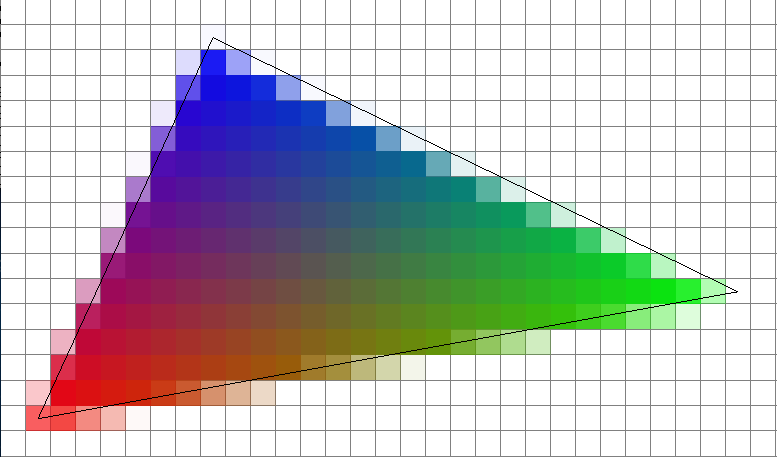
\includegraphics[width=0.65\textwidth]{graphics/df/rasterization}
	\caption{By resterization, a parametric surface is only need to record a small group of points of the surface. More point's position will be interpolated in the resterization stage of the rendering pipeline.}
	\label{f:resterization}
\end{figure}

I guess that's why rasterization so popular. Because we only need to iterate each point of the surface and calculate it's color, which is performed by computing the lighting effect in the rendering equation. This is called local illumination because it only consider the direct reflections. 

But in the real world the indirect lighting is even more important. Lack of indirect lighting, the surface which can not see the light directly will be totally dark. This of course is not realistic. So people invented some technology to simulate these phenomenons, such as ambient light, environment light and sky light etc, which can be precomputed to a texture and can be mapped to the surface. That's means we still don't need to interact with other points of the surface in the scene.   

Unfortunately, we still need to count the interactions between points. When the objects moved dynamically, the precomputed maps could not be used any more. The real world is always changing, the character is moving, the sky light is changing, and the wind is shaking the trees etc. As a result, the lights and shadows are all changed.

\begin{figure*}\label{f:object-mobility}
	\begin{subfigure}[b]{0.49\textwidth}
		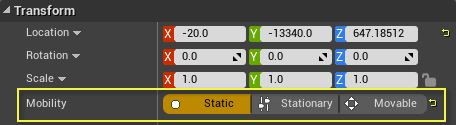
\includegraphics{graphics/df/IL_mobility}
		\caption{Light Mobility}
	\end{subfigure}
	\begin{subfigure}[b]{0.51\textwidth}
		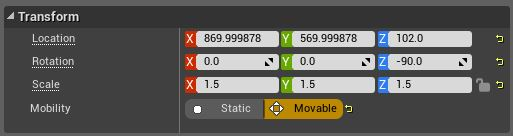
\includegraphics{graphics/df/TransformMobility}
		\caption{Actor Mobility}
	\end{subfigure}
	\caption{In Unreal Engine 4, every light and actor has its 'mobility' property. So the engine can decide which objects' light and shadow calculation can be precomputed.}
\end{figure*}

In a scene, usually only few objects are dynamic, like characters and cars. Many game engine (like Unreal Engine 4 in figure \ref{f:object-mobility}) provide a mobility property for the objects. So the dynamic computation can be reduced by only counting these small dynamic objects. That really can improve performance a lot. All static or stationary objects can have some degree of pre-computing.

Lastly, the few dynamic objects and the phenomenons which must be calculated dynamically, such as the ambient occlusion from the movable sky light, we provide another representation of the surface to handle them. That's why we need Implicit Surfaces.

\section{Implicit Surfaces}

You might wander why I kept on talking about rasterization. Because that's the very important part to understand implicit surfaces. We introduce implicit surfaces to solve the very important problem --- ray-surface intersection calculation. Most of the applications of distance field we will explain in this article, such as ambient occlusion, destruction mask etc, they all have the same essential problem: they need to calculate ray-surface dynamically. So as an addition to parametric surfaces, implicit surface is introduced to computer graphics to mainly solve the ray-surface intersection calculation.

An \textit{implicit surface} is the collection of all points $P$ satisfying an implicit equation of the form $F(P)=0$. Typically, the function $F$ is a polynomial in coordinates $x,y$ of the points $P$. For example, a unit circle can be represented by the implicit equation: 

\begin{equation*}
	F(x,y)\equiv x^2+y^2=0
\end{equation*}

We refer to $\Omega^-=\{\vec{x}||\vec{x}|<1\}$ as the \textit{inside} portion of the domain and $\Omega^+=\{\vec{x}||\vec{x}|>1\}$ as the \textit{outside} portion of the domain. The border between the inside and the outside consists of the circle $\partial\Omega=\{\vec{x}||\vec{x}|=1\}$\footnote{Here symbol $\partial$ means boundary. $\partial M$ means the boundary of $M$. Examples: $\partial \{x:|x|\leq 2\}=\{x:|x|=2\}$.} and its called the \textit{interface}.

\textbf{Generally, in $R^n$, the interface has dimension $n-1$.} We say that the interface has codimension one. For example, in parametric representation, a circle has one parameter so its one dimension; a sphere in tree spatial dimension can be represented by two parameter: $P=P(s,t)$, so its two dimension.

But an implicit interface representation defines the interface as the ioscontour of some function. For example, the zero ioscontour of $\phi(x,y)=x^2+y^2-1$ is the set of all points where $\phi(x,y)=0$; it is exactly $\partial\Omega=\{\vec{x}||\vec{x}|=1\}$. This is shown in figure \ref{f:implicit-function}. Here the implicit function $\phi(x,y)$ is defined throughout the two dimension domain, while the ioscontour defining the interface is one dimension. \textbf{More generally, in $R^n$, the implicit function $\phi(\vec{x})$ is defined on all $\vec{x}\in R^n$, and its isocontour has dimension $n-1$.}

\begin{figure}\label{f:implicit-function}
	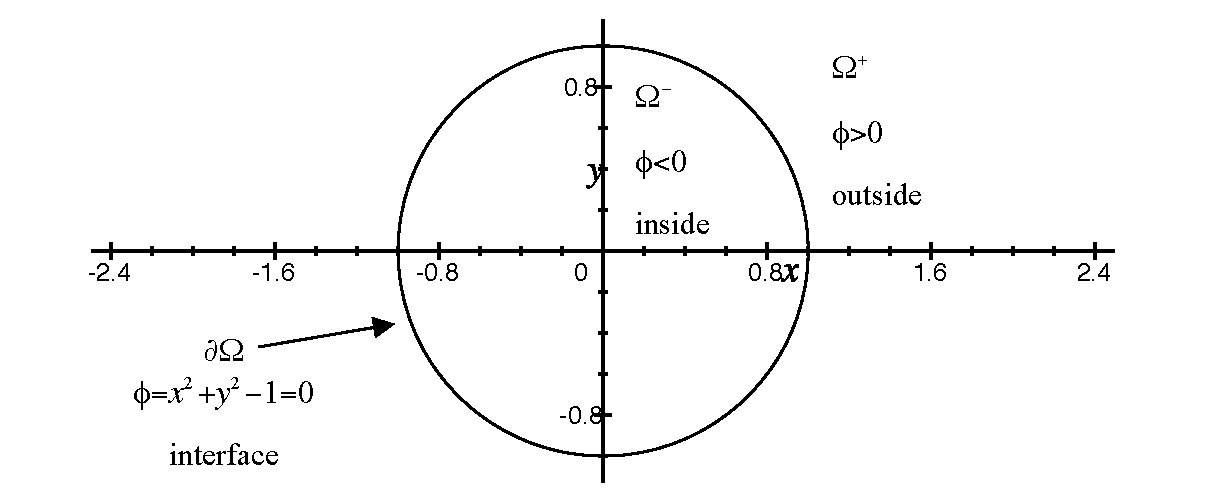
\includegraphics{graphics/df/implicit-function}
	\caption{Implicit function $\phi(x,y)=x^2+y^2-1$ defining the regions $\Omega^-$ and $\Omega^+$ as well as the boundary $\partial\Omega$}
\end{figure}

So, to represent implicit surfaces, we need more spaces to store the points, since the implicit function $\phi(\vec{x})$ is defined on all $R^n$, while the interface has only dimension $n-1$. However, we could use some methods to save spaces. 




\subsection{Basic Property}
Since $\phi(\vec{x})$ is defined on all $\vec{x}\in R^n$, we can easily determine if a point $\vec{x}$ lies on an implicit surface. Here we only need check if $\phi(\vec{x})=0$. Moreover,points on different sides of an implicit surface are distinguished by the sign of $\phi$; for closed surfaces:

\begin{figure}
\sidecaption
	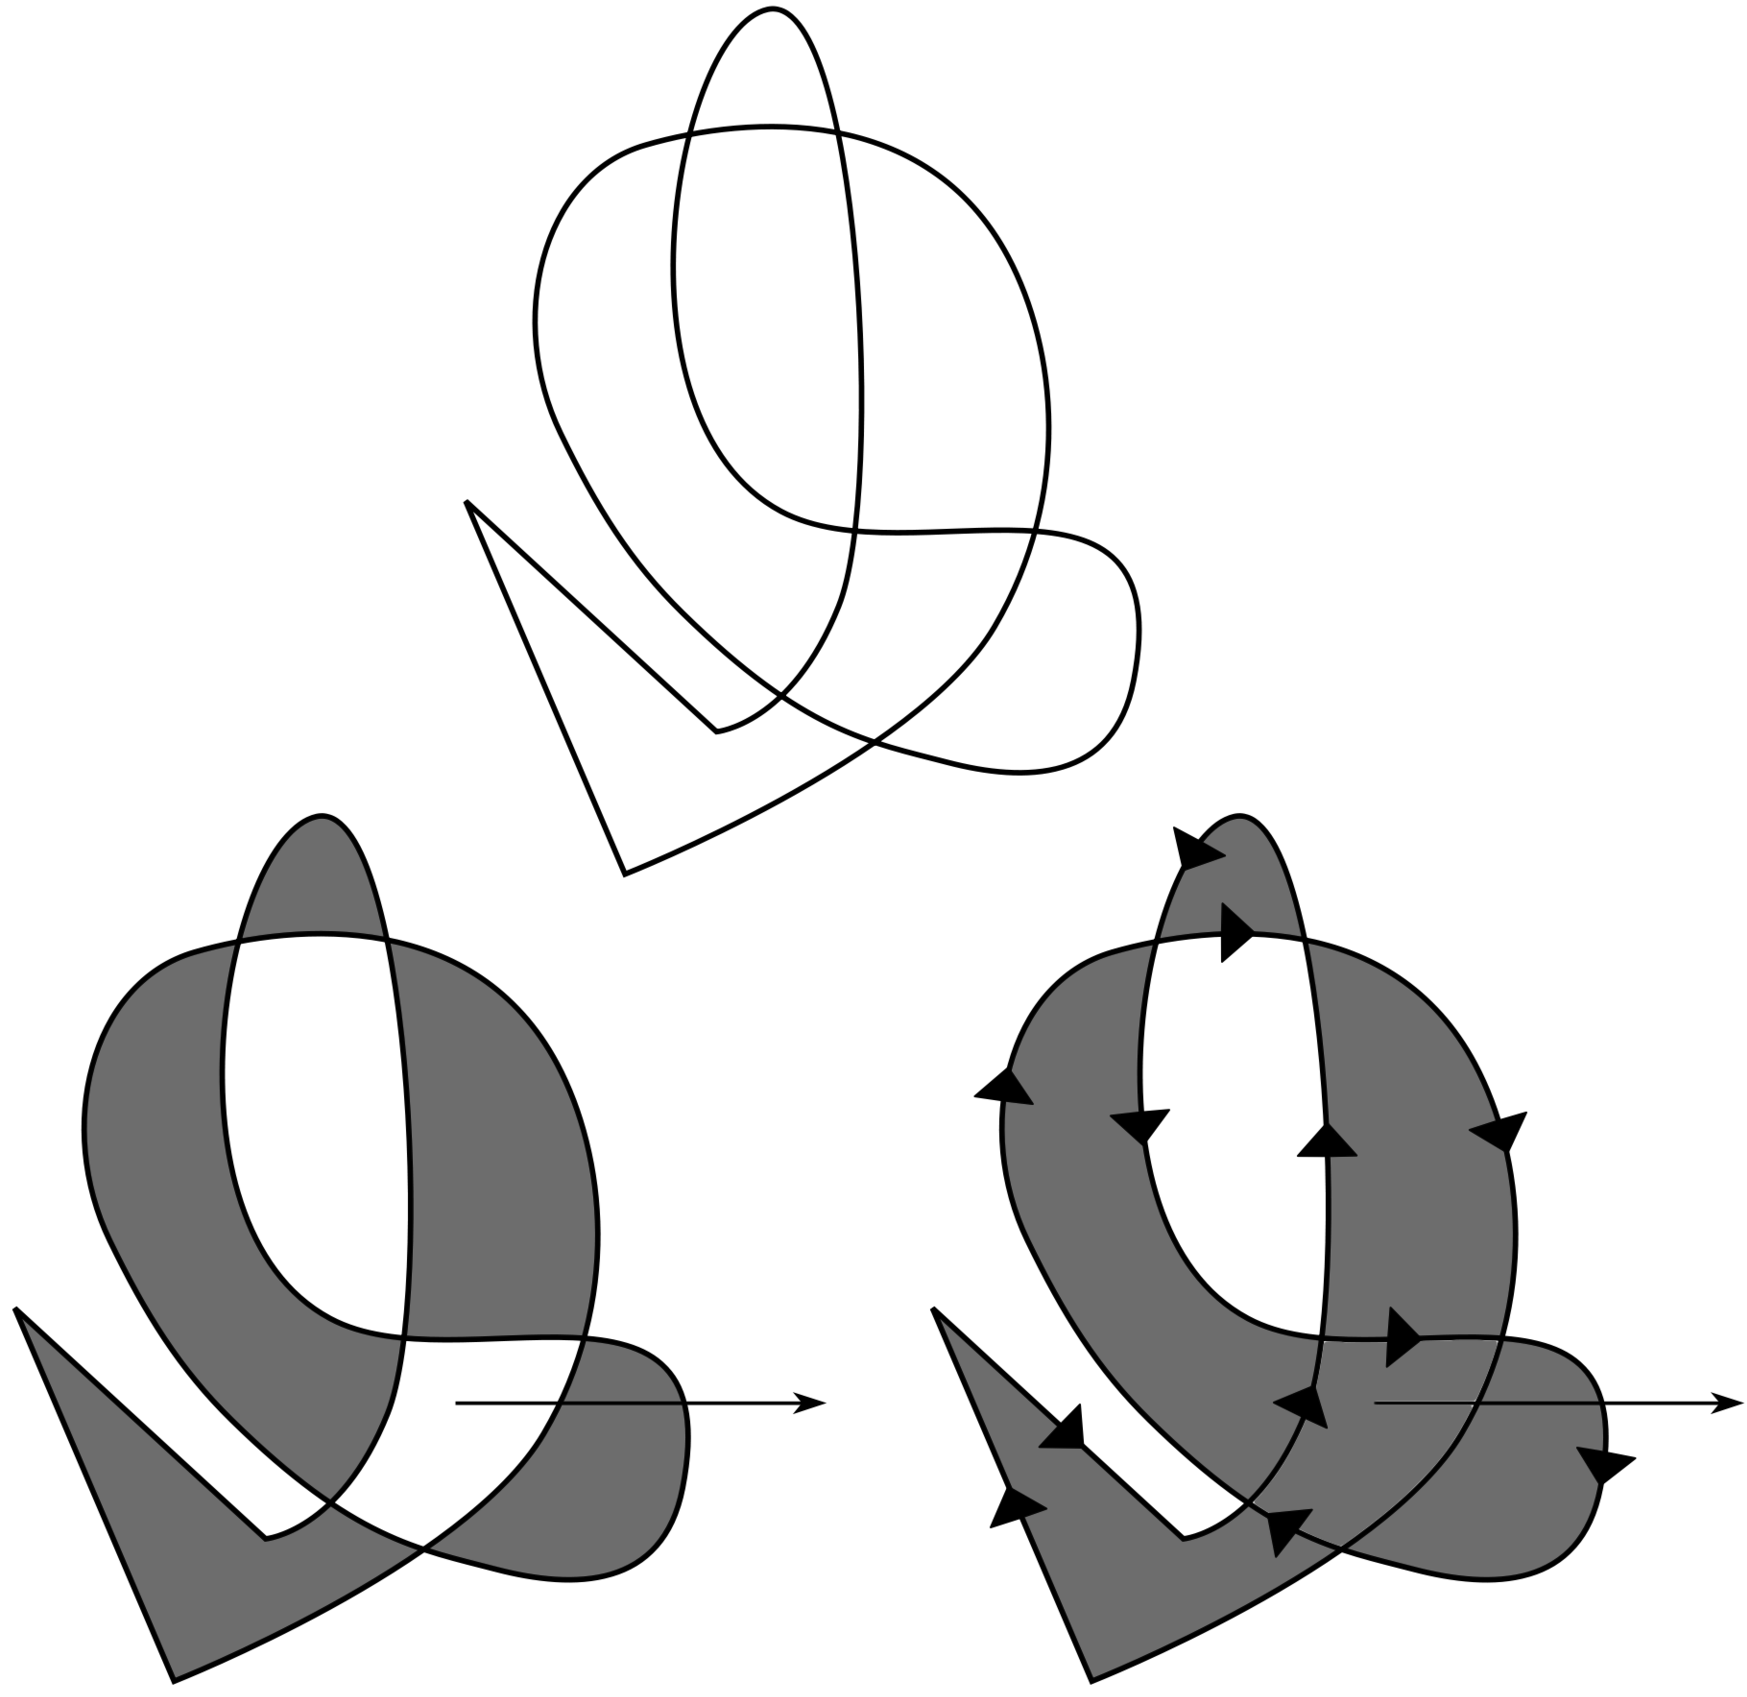
\includegraphics[width=.65\textwidth]{graphics/df/Even-odd_and_non-zero_winding_fill_rules}
	\caption{A curve (top) is filled according to two rules: the even-odd rule (left), and the non-zero winding rule (right). In each case an arrow shows a ray from a point P heading out of the curve. In the even-odd case, the ray is intersected by two lines, an even number; therefore P is concluded to be 'outside' the curve. By the non-zero winding rule, the ray is intersected in a clockwise direction twice, each contributing -1 to the winding score: because the total, -2, is not zero, P is concluded to be 'inside' the curve(Images courtesy of Wikipedia)}.
\end{figure} 

\begin{equation*}
	\phi(\vec{x})=
	\begin{cases}
    <0,& \text{if } \vec{x}\in\Omega^-\\
    =0, & \text{if } \vec{x}\in\partial\Omega\\
    >0,&\text{if } \vec{x}\in\Omega^+
\end{cases}
\end{equation*}   

This can also be figured out from figure \ref{f:implicit-function}. The distance function we will talk in the next section also satisfies this condition.

With an explicit representation of the interface it can be difficult to determine whether a point is inside or outside the interface. Since it has dimension $n-1$, there lacks lots of informations about the space. A standard procedure for doing this is to cast a ray from the point in question to some far-off place that is known to be outside the interface. Then if the ray intersects the interface an even number of times, the point is outside the interface. Otherwise, the ray intersects the interface an odd number of times, and the point is inside the interface. this is called \textit{even-odd rule}. Another available method is \textit{non-zero winding rule}.


\subsection{Surface Normals}
For an implicit surface $\phi(\vec{x})=0$, the normal vector $N$ is given by gradient---that is,

\begin{equation}\label{e:implicit-surface-gradient}
	\vec{N}=\bigtriangledown\phi=(\frac{\partial\phi}{\partial{x}},\frac{\partial\phi}{\partial{y}},\frac{\partial\phi}{\partial{z}})
\end{equation}

The book \cite{b:AnIntegratedIntroductiontoCG} provided a proof use the chain rule. Suppose that $P(t)=(x(t),y(t),z(t))$ is a parametric curve on the surface $\phi(\vec{x})=0$. Then

\begin{equation*}
	\phi (x(t),y(t),z(t))=0
\end{equation*}

Hence, by the chain rule,

\begin{equation*}
		\frac{\partial\phi}{\partial{x}}\frac{dx}{dt}+\frac{\partial\phi}{\partial{y}}\frac{dy}{dt}+\frac{\partial\phi}{\partial{z}}\frac{dz}{dt}=\frac{d\phi}{dt}=0
\end{equation*} 

Therefore,

\begin{figure}
\sidecaption
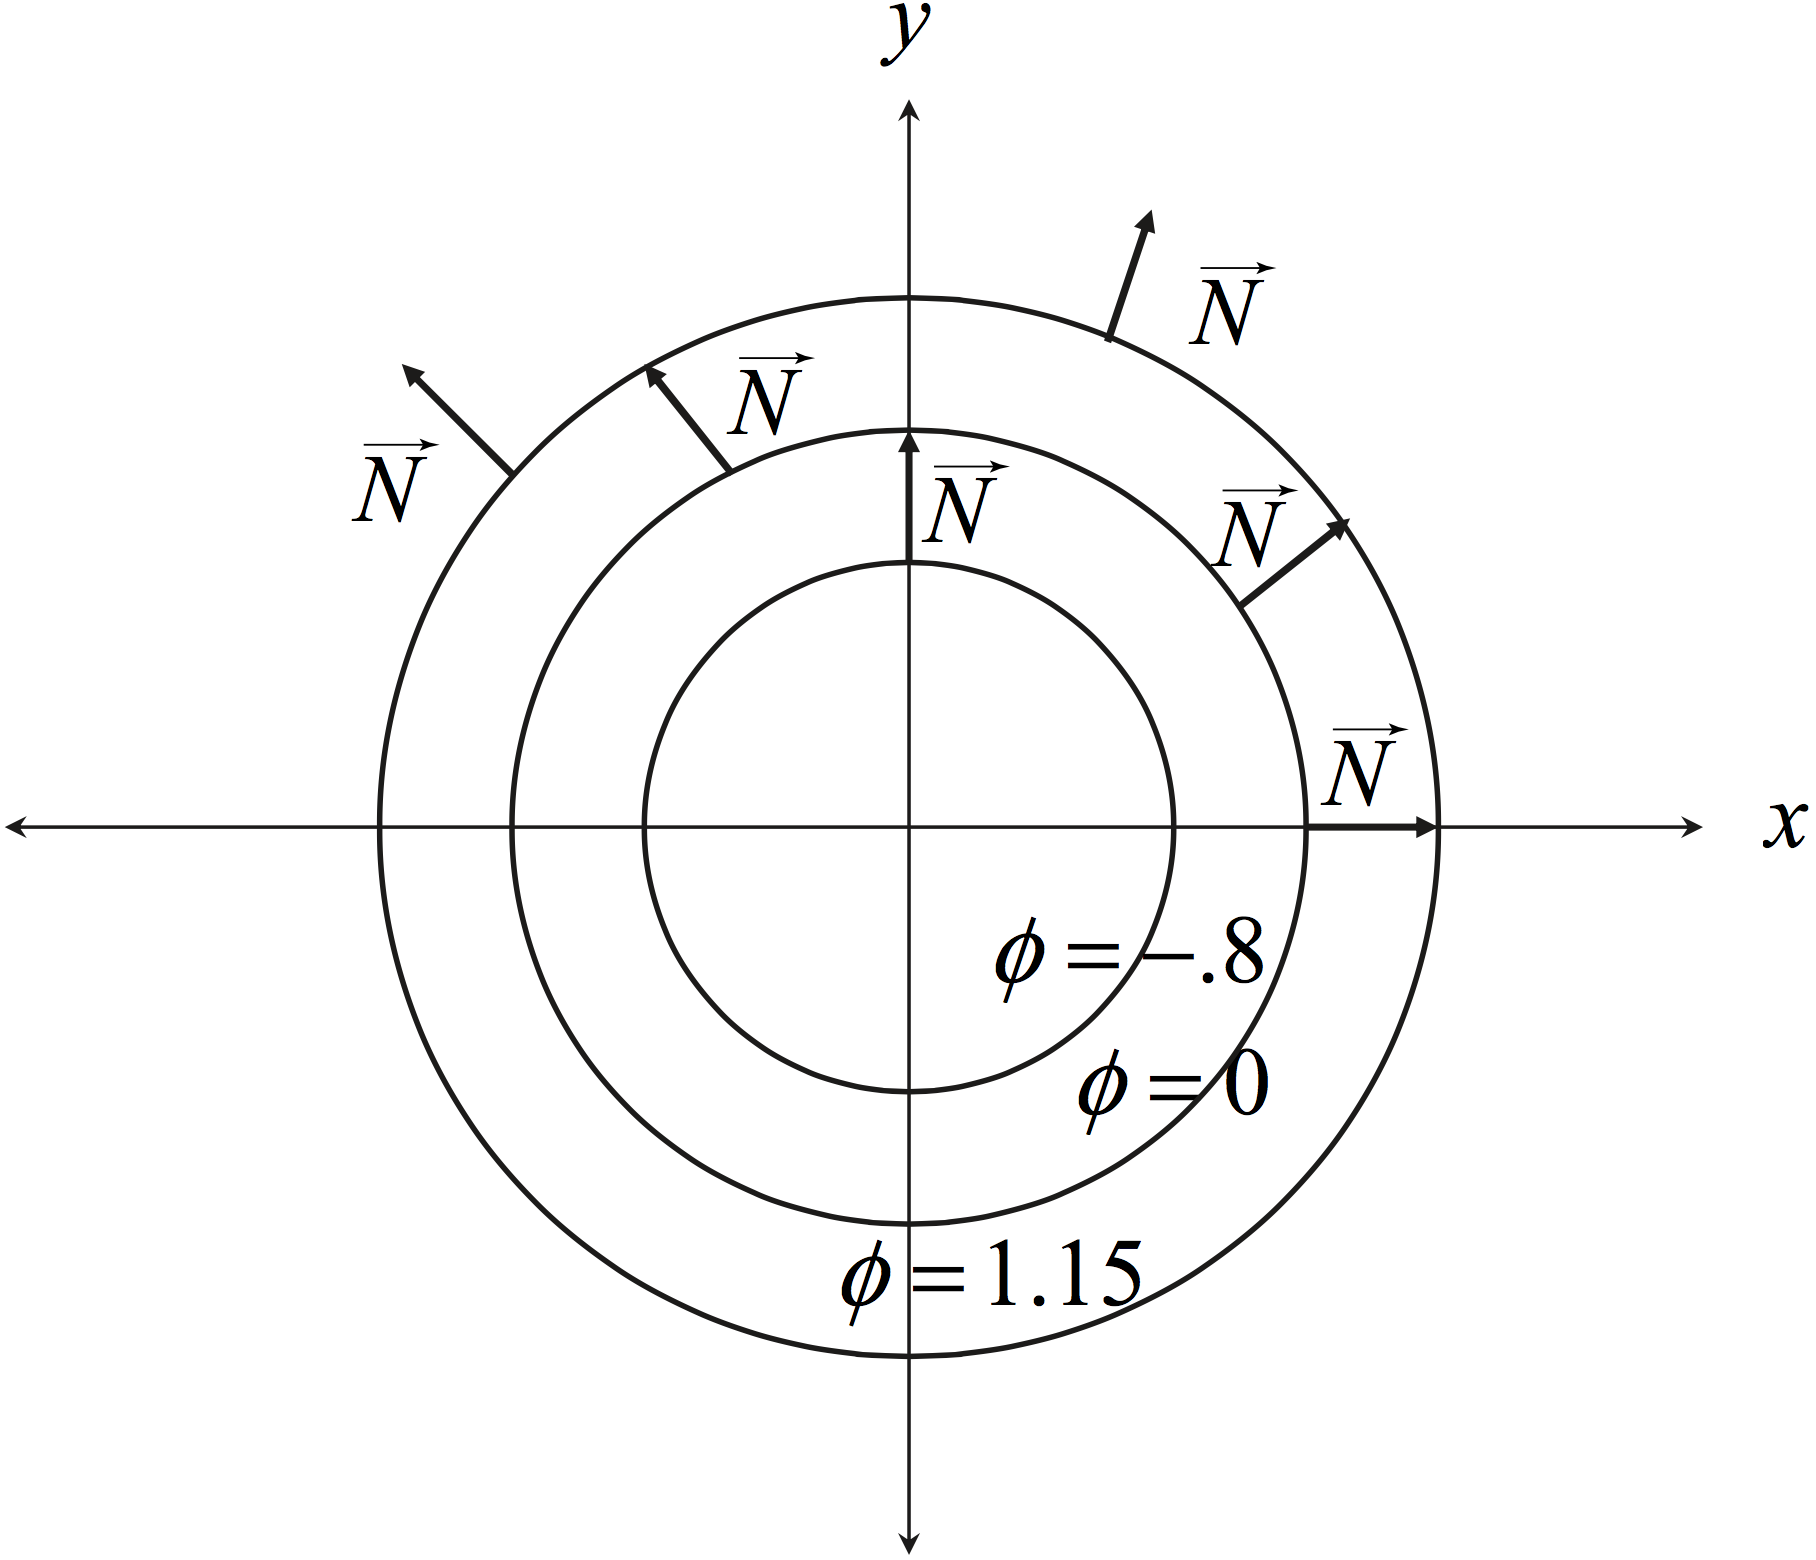
\includegraphics[width=0.65\textwidth]{graphics/df/gradient-of-implicit-function}
\caption{A few isocontours of our two-dimensional example $\phi(\vec{x})=x^2 + y^2-1$
along with some representative normals.}	
\end{figure}

\begin{equation*}
	\underbrace{\bigtriangledown\phi}_{\text{Gradient}}\cdot\underbrace{P^{'}(t)}_{\text{Derivative}}=\underbrace{(\frac{\partial\phi}{\partial{x}},\frac{\partial\phi}{\partial{y}},\frac{\partial\phi}{\partial{z}})}_{\text{Normal vector}}\cdot\underbrace{(\frac{dx}{dt},\frac{dy}{dt},\frac{dz}{dt})}_{\text{Tangent vector}}=0
\end{equation*}

So

\begin{equation*}
	\vec{N}=\bigtriangledown\phi=(\frac{\partial\phi}{\partial{x}},\frac{\partial\phi}{\partial{y}},\frac{\partial\phi}{\partial{z}})
\end{equation*}


Since the implicit representation of the interface embeds the interface in a domain of one higher-dimension, it will be useful to have as much information as possible representable on the higher-dimensional domain. For example, instead of defining the unit normal $\vec{N}$ for points on the interface only, we use equation \ref{e:implicit-surface-gradient} to define a function $\vec{N}$ everywhere on the domain. This embeds the normal in a function $\vec{N}$ defined on the entire domain that agrees with the normal for points on the interface.

\subsection{Boolean Operations}
Implicit functions make both simple Boolean operations and more advanced \textit{constructive solid geometry (CSG)} operations easy to apply. This is important, for example, in computer-aided design (CAD). If $\phi_1$ and $\phi_2$ are two different implicit functions, then $\phi(\vec{x})=min(\phi(\vec{x})_1,\phi(\vec{x}_2))$ is the implicit function representing the union of the interior regions of $\phi_1$ and $\phi_2$. Similarly, $\phi(\vec{x})=max(\phi(\vec{x})_1,\phi(\vec{x}_2))$ is the implicit function representing the intersection of the interior regions of $\phi_1$ and $\phi_2$. The complement of $\phi(\vec{x})_1$ can be defined by $\phi(\vec{x})=-\phi(\vec{x})_1$. Also, $\phi(\vec{x})=max(\phi(\vec{x})_1,-\phi(\vec{x}_2))$ represents the region obtained by subtracting the interior of $\phi_2$ from the interior of $\phi_1$.

\begin{figure}
	\begin{center}
		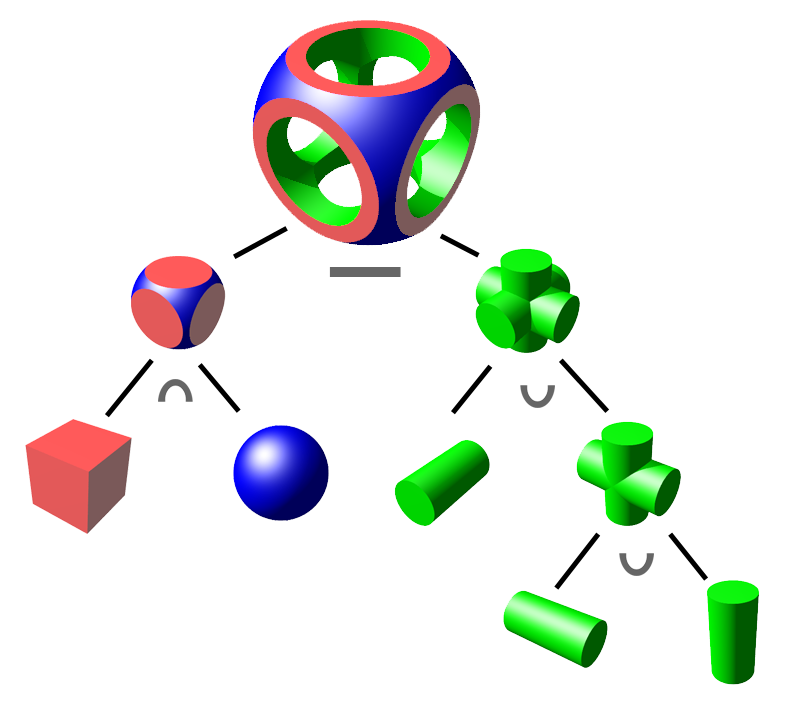
\includegraphics[width=0.6\textwidth]{graphics/df/Csg-tree}
	\end{center}
	\caption{CSG objects can be represented by binary trees, where leaves represent primitives, and nodes represent operations. In this figure, the nodes are labeled for intersection, for union, and for difference(Images courtesy of Wikipedia).}
\end{figure}

In the next section, we will introduce the boolean operations of signed distance functions. 




\section{Signed Distance Functions}
In the last section we have defined implicit functions with $\phi(\vec{x})\leq 0$ in the interior region $\Omega^-$, $\phi(\vec{x})\geq 0$ in the exterior region $\Omega^+$, and $\phi(\vec{x})=0$ on the boundary $\partial\Omega$. But what dose a implicit function look like? In this section we will discuss \textit{signed distance functions} which are a subset of implicit functions. That is the value of the function is positive on the exterior, negative on the interior, and zero on the boundary. 

A \textit{distance function} $d(\vec{x})$ is defined as 

\begin{equation}
	d(\vec{x})=min(|\vec{x}-\vec{x}_{I}|)  
\end{equation}

\begin{figure}
\sidecaption
	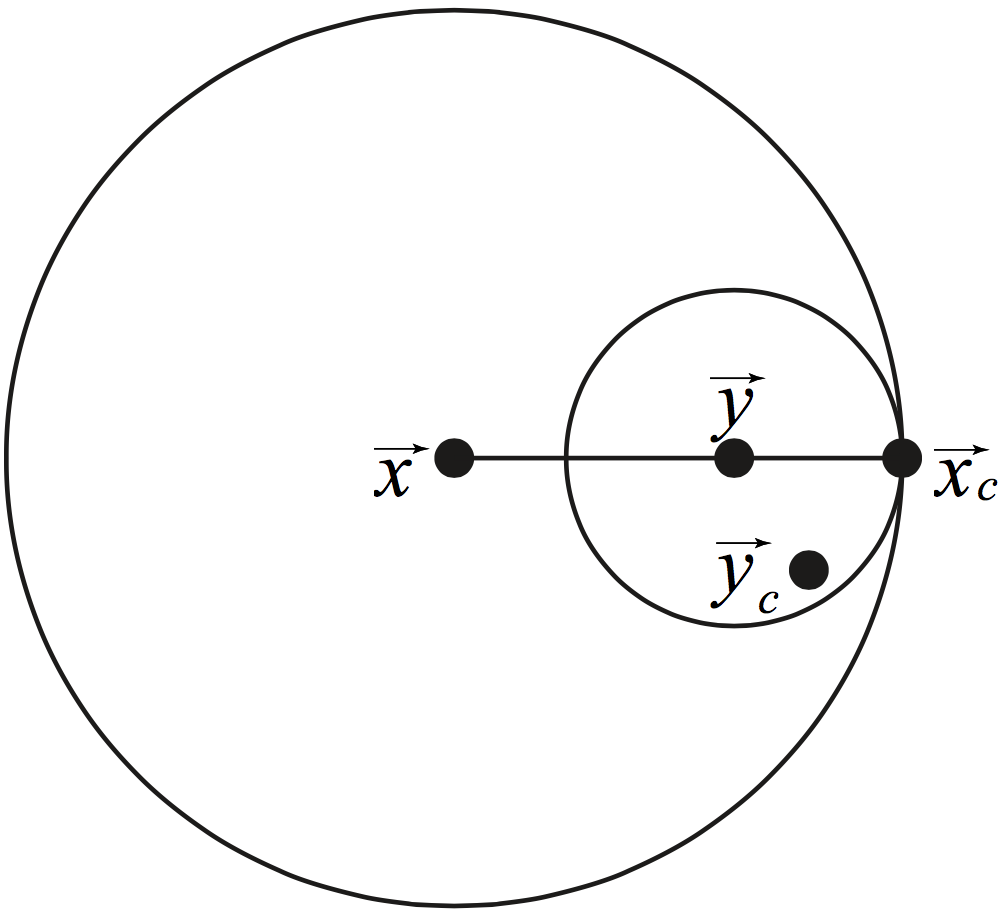
\includegraphics[width=0.65\textwidth]{graphics/df/distance-function}
	\caption{$\vec{x}_C$ is the closest interface point to $\vec{{x}}$ and $\vec{y}$.}
\end{figure}

for all $\vec{x}_{I}\in\partial\Omega$, which implies that $d(\vec{x})=0$ on the boundary where $\vec{x}\in\partial\Omega$. Geometrically, d may be constructed as follows. If $\vec{x}\in\partial\Omega$, then $d(\vec{x}) = 0$. Otherwise, for a given point $\vec{x}$, find the point on the boundary set $\partial\Omega$ closest to $\vec{x}$, and label this point $\vec{x}_C$ . Then $d(\vec{x}) = |\vec{x} - \vec{x}_C |$.

A \textit{signed distance function} is an implicit function $\phi$ with $|\phi(\vec{x})| = d(\vec{x})$ for all $\vec{x}$ . Thus , $\phi(\vec{x}) = d(\vec{x})=0$ for all $\vec{x}\in\partial\Omega$, $\phi(\vec{x})=-d(\vec{x})$ for all $\vec{x}\in\Omega^-$, and $\phi(\vec{x}) = d(\vec{x})$ for al $\vec{x}\in\Omega^+$. Signed distance functions share all the properties of implicit functions discussed in the last section.

Inigo Quilez has provided some distance functions for basic primitives in his website\footnote{Modeling with distance functions: \url{http://iquilezles.org/www/articles/distfunctions/distfunctions.htm}}. He also given the code you could use on the shader or somewhere else. Such as the signed distance function of Sphere.

\begin{table}
\begin{tabular}{m{3.0cm}m{7.cm}} 
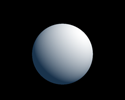
\includegraphics{graphics/df/sphere} &
	 \begin{lstlisting}
Sphere - signed:
float sdSphere(vec3 p, float s)
{
  return length(p)-s;
}
\end{lstlisting} \\
   
\includegraphics{graphics/df/torus} & 
    \begin{lstlisting}
Torus - signed:
float sdTorus(vec3 p, vec2 t )
{
  vec2 q = vec2(length(p.xz)-t.x,p.y);
  return length(q)-t.y;
}
   \end{lstlisting}
\end{tabular}
\caption{Two examples of distance functions of basic primitives(Images courtesy of http://iquilezles.org)}
\end{table}

As aforementioned, it's easy to do boolean operations between implicit functions. Inigo Quilez also provided several functions to combine distance functions:

\begin{table}
\begin{tabular}{m{3cm}m{7.cm}} 
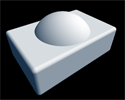
\includegraphics{graphics/df/union} &
	 \begin{lstlisting}
Union:
float opU(float d1, float d2)
{
    return min(d1,d2);
}
\end{lstlisting} \\
   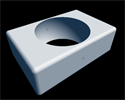
\includegraphics{graphics/df/substraction} & 
    \begin{lstlisting}
Substraction:
float opS(float d1, float d2)
{
    return max(-d1,d2);
}
   \end{lstlisting}
\end{tabular}
\caption{The d1 and d2 parameters in the following functions are the distance to the two distance fields to combine together(Images courtesy of http://iquilezles.org).}
\end{table}

Inigo Quilez also provided some distance deformations. We will go further about these topics in the next sections. 

Given a signed distance function, we could get any point's distance from the closest surface, which can be used in ray-marching or sphere-tracing we will introduce in section \ref{s:rendering-of-implicit-surfaces}. Further more, using Inigo Quilez's functions we could get the distance function from a explicit representation.  

But the real world is more complex than these. Such as the object maybe consists of thousands of triangles, it can be very complicate. We might precomputed the distance fields to volume texture, or compute it in GPU in real time, or compute it from fractals. We will discuss the scene presentation more deeply in the next section.  

\begin{figure}\label{f:object-mobility}
	\begin{subfigure}[b]{.50\textwidth}
		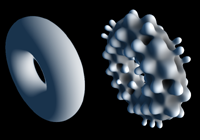
\includegraphics{graphics/df/displacement}
		\caption{Displacement}
	\end{subfigure}
	\begin{subfigure}[b]{.50\textwidth}
		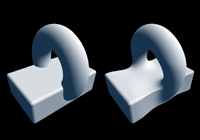
\includegraphics{graphics/df/blend}
		\caption{Blend}
	\end{subfigure}
	\caption{Distance deformations, the displacement example us using sin(20*p.x)*sin(20*p.y)*sin(20*p.z) as displacement pattern(Images courtesy of http://iquilezles.org).}
\end{figure}









\chapter{Scene Representation}
In this section, we will talk about the representation of implicit surfaces. Specifically, we only talk about the distance field representation. First we will discuss methods are used to compute distance fields; and secondly, how is the distance field data stored in GPU; and lastly we will discuss methods are used to compute distance field dynamically in GPU in real time.  

\section{Computing Distance Fields}
A brute-force algorithm for computation of a shortest distance to a set of objects over a 3D discrete grid $\nu$ is very simple: for each voxel of $\nu$ its distance to all objects is computed, by tracing rays in all directions to find the nearest surface, and the smallest one is stored. Unreal Engine 4 used this method to generate offline distance fields.

\begin{figure}
\sidecaption
	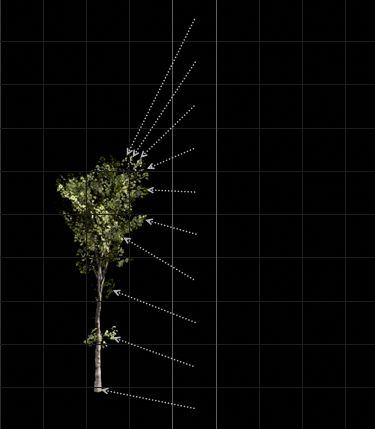
\includegraphics[width=0.65\textwidth]{graphics/df/brute-force-method}
	\caption{Mesh SDF generated offline with brute force triangle raytracing in Unreal Engine 4.}
\end{figure}

In spite of it's simplicity, this approach is time-consuming and impractical. The other practical approaches can be divided into two categories:

\begin{enumerate}
	\item trying to discard most of the objects which probably farther than other spatial coherency objects and 
	\item methods, which in an initialization step evaluate the distances in certain regions in a trivial way (inside the objects or in a thin layer around the surface) and subsequently propagate them through the whole volume (distance transforms).
\end{enumerate}

These methods have a fast computation time but a less accurate results. In the real situation, brute-force techniques can be used to precompute high accurate offline SDF(like the Unreal Engine 4 case) for static objects, and these accelerated techniques could be used for few dynamic objects in run time. There are also methods to compute SDFs fast enough at runtime in Unreal Engine 4.





\section{SDF for Common Surface Representations}
\begin{figure}
\sidecaption
	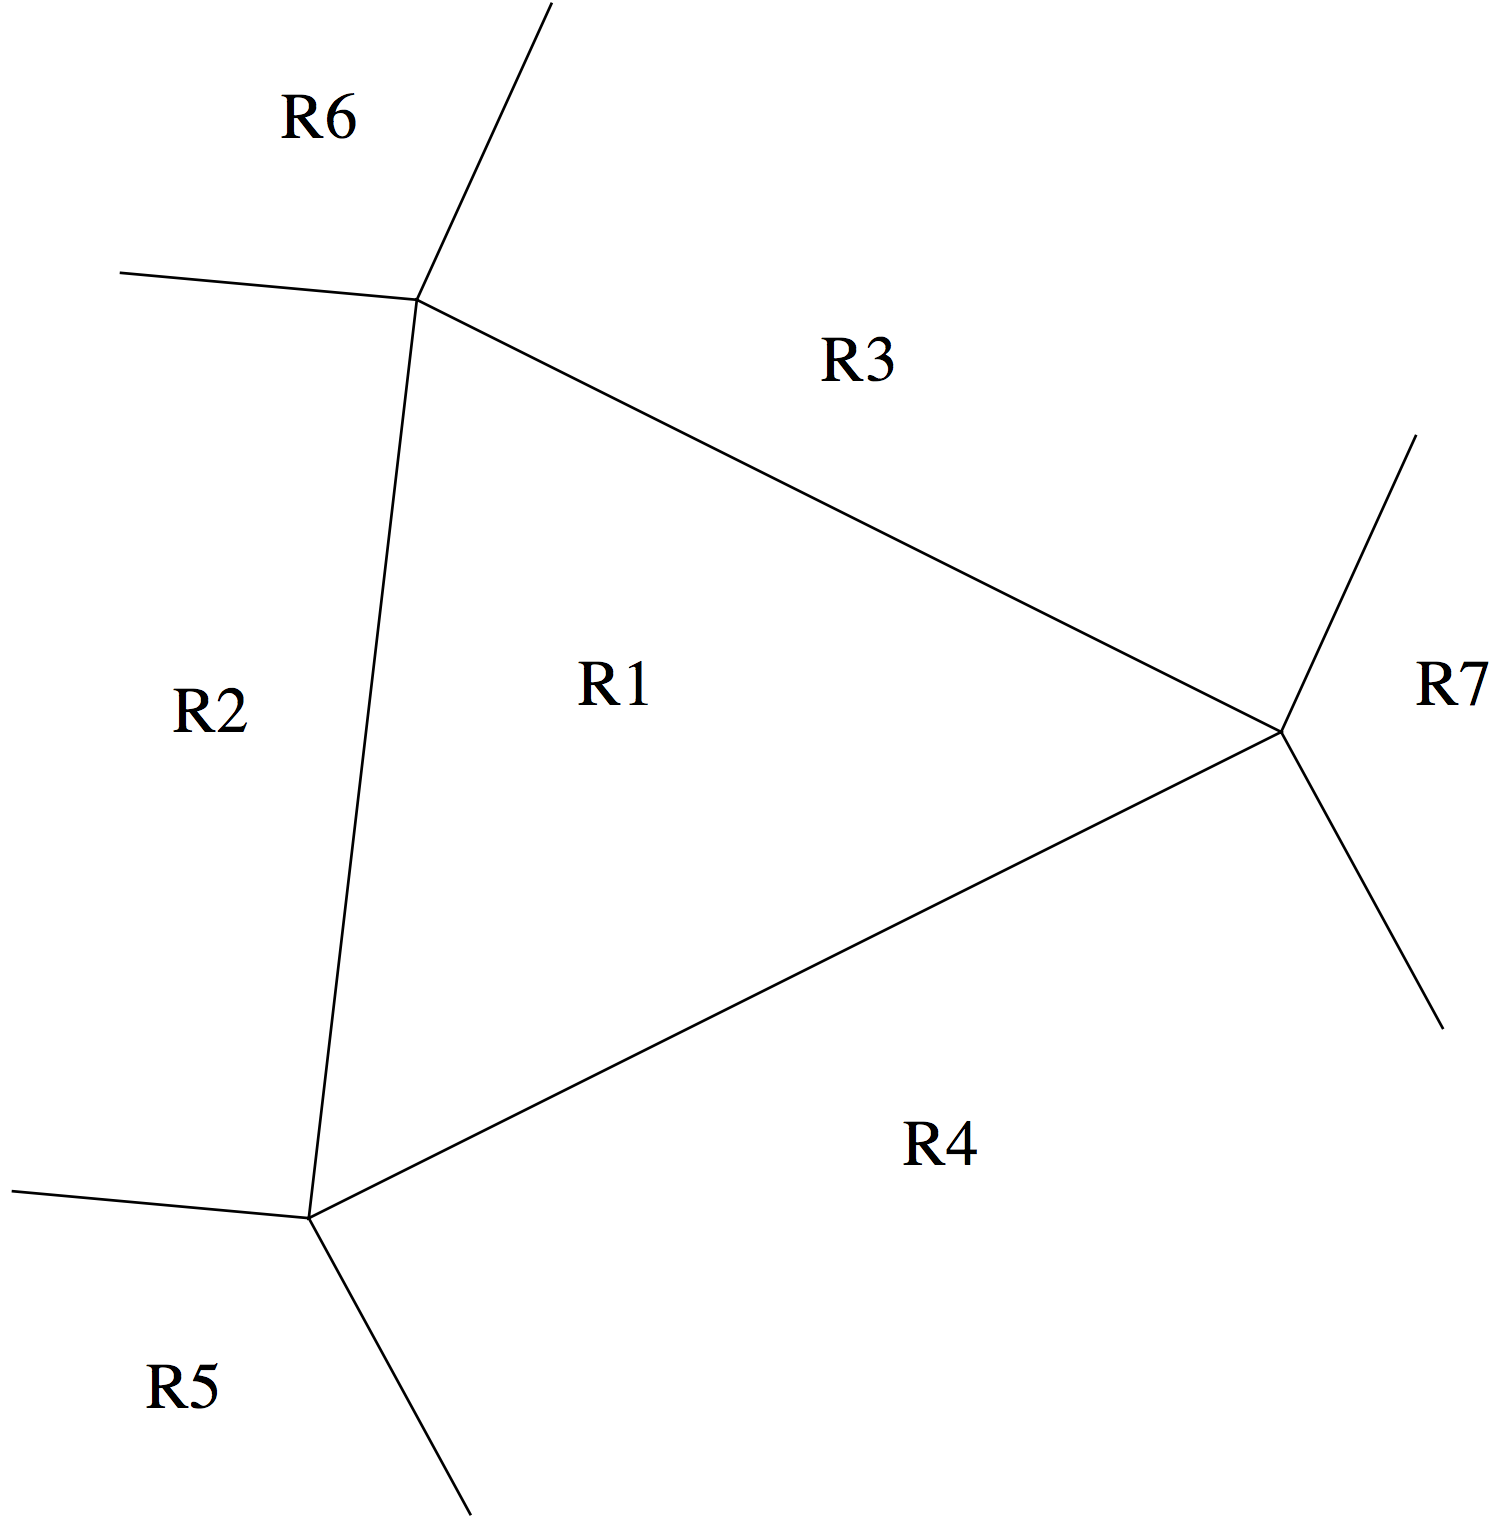
\includegraphics[width=0.65\textwidth]{graphics/df/calculating-distance-to-triangle}
	\caption{Calculating distance to a triangle: If $p$ projects onto $R1$ it is closest to the plane, $R2-R4$ edge, $R5-R7$vertex.}
	\label{f:triangle-distance}
\end{figure}

The triangle mesh representation is probably the most frequently used in representation for 3D geometry. Therefore, it is particularly important that we are able to convert triangle meshes to signed distance fields. We can only generate distance fields from a certain class of triangle meshes, namely meshes that are closed, orientable 2-manifolds.

The distance to a triangle is easily computed using a simple case analysis. When a point $p$ is projected onto the plane containing the triangle, the projected point $p^{'}$ lies in one of the 7 regions shown in figure \ref[5mm]{f:triangle-distance}. If $p^{'}$ is projected onto R1 then the distance from the point to the triangle is equal to the distance from the point to the plane containing the triangle. If $p^{'}$ lies in R2, R3 or R4 a distance to the corresponding line should be calculated. Lastly, with regions R5, R6 or R7 a distance to the corresponding vertex should be calculated(see \cite[-20mm]{a:3d-distance-fields-a-survey}).

The brute force method requires $N\cdot M$ steps, where $N$ is the number of voxels, and $M$ is the number of triangles, it is sensible to use hierarchical data structures to allow $O(logM)$ access to the triangles.

\begin{figure}
\sidecaption
	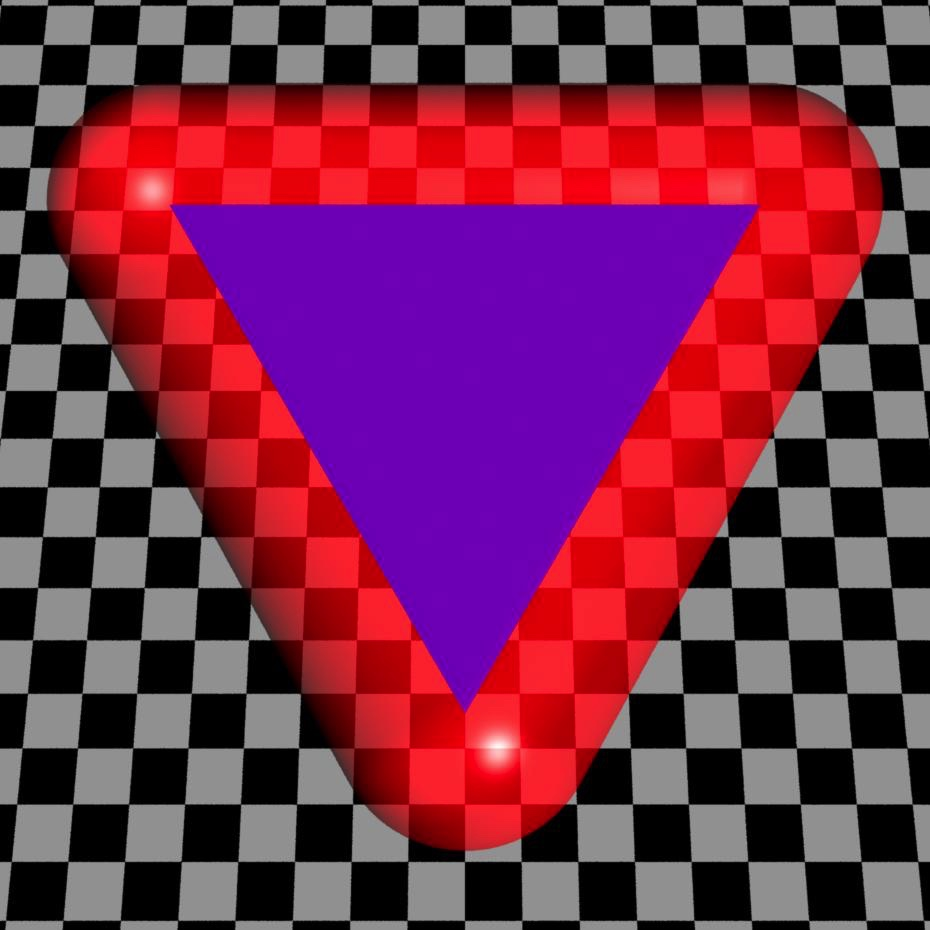
\includegraphics[width=0.65\textwidth]{graphics/df/close-triangle}
	\caption{The 3D region of influence around a triangle}
	\label{f:close-triangle}
\end{figure}

Sometimes, only the value up to a certain distance from the surface is required. We can use a bounding volume around each triangle to ensure that distance are only computed for grid points that are potentially closer than some distances. See figure \ref{f:close-triangle}. The approach can be found in \cite[5.0mm]{a:Incremental-Triangle-Voxelization}.

After computed the distance field, we need to compute the sign. The most obvious method for computing the sign when generating a signed distance field is to use the surface normals. If we have a $C^{1}$ smooth surface, the sign of the distance can be found by evaluating the dot product of the normal, n and a direction vector, d from the closest point to the point p where the sign is desired. d will always point either in the same direction as n (if we are outside) or the opposite (if we are inside).

\begin{figure}
\sidecaption
	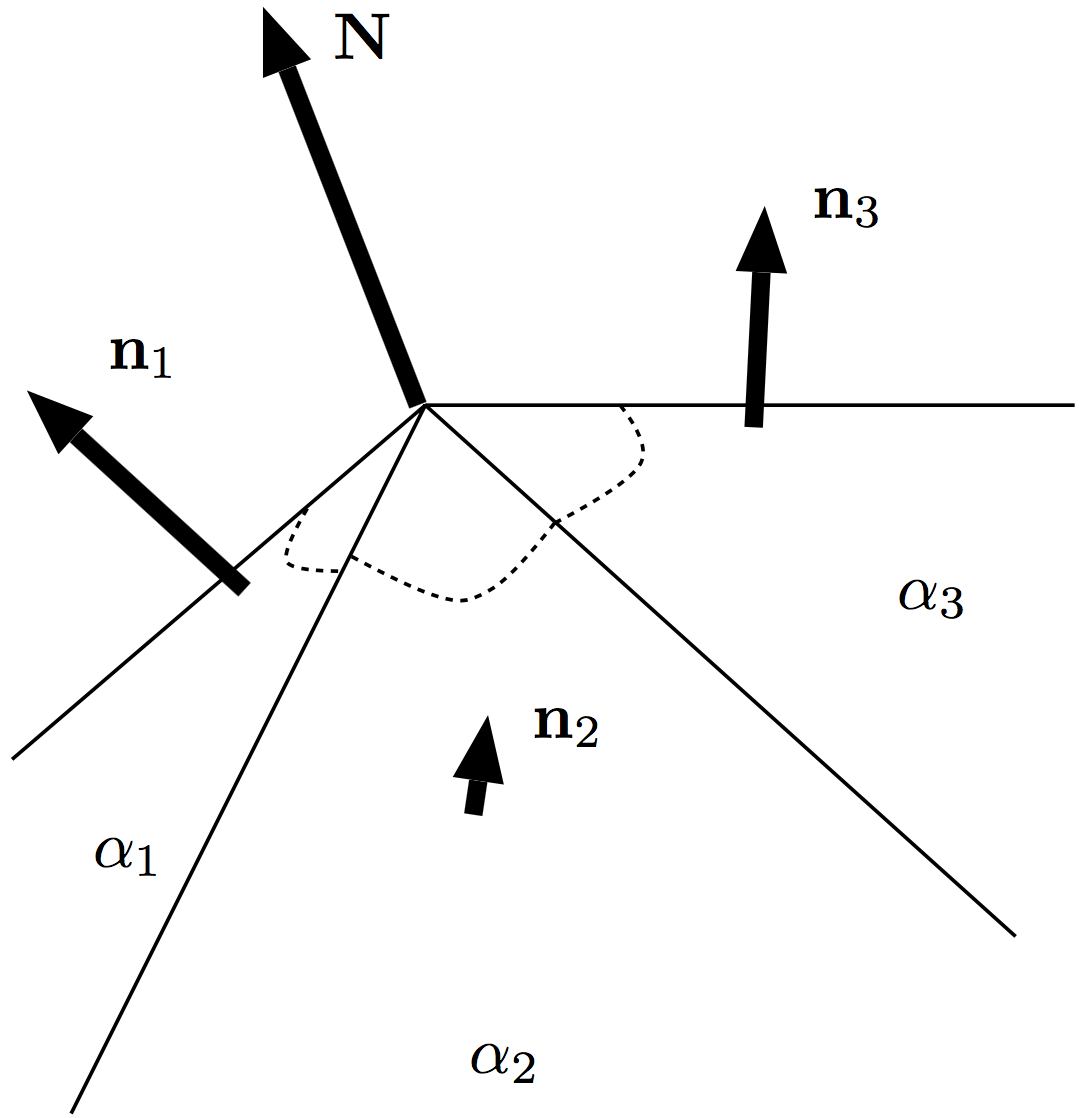
\includegraphics[width=0.65\textwidth]{graphics/df/Computing-vertex-normals}
	\caption{The angle weighted normal $N=\frac{\sum_{i}n_{i}a_{i}}{||\sum_{i}n_{i}a_{i}||}$}
	\label{f:weighted-normal}
\end{figure}


The problem with triangle meshes is that they are not $C^{1}$: The normal is not defined on edges and vertices. Aanaes and Baerentzen use the angle weighted normal as a pseudo normal at the vertex and edge. To compute the angle weighted normal at a vertex, one sums the normals of the incident faces, weighting each normal with the angle between the two legs that are incident to the vertex, see figure \ref{f:weighted-normal}.


Computing the sign can be challenging for arbitrary unclosed meshes. For Unreal Engine 4, A simple heuristic that works well for determining 'inside': after tracing rays to find the closest surface, if the number of backface hits is >50\% of the rays traced, that position is inside. See figure \ref{f:ue4-sign}: 

\begin{figure}\label{f:ue4-sign}
	\begin{subfigure}[b]{0.5\textwidth}
		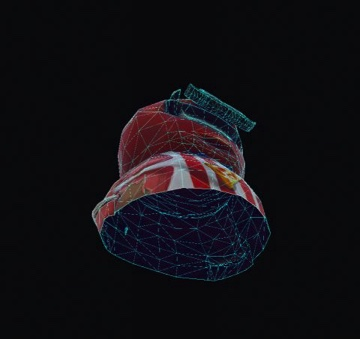
\includegraphics{graphics/df/ue4-sign-1}
		\caption{A unclosed mesh}
	\end{subfigure}
	\begin{subfigure}[b]{0.5\textwidth}
		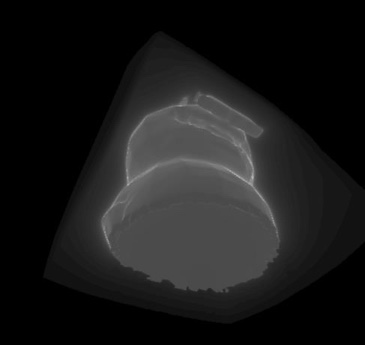
\includegraphics{graphics/df/ue4-sign-2}
		\caption{It's distance field}
	\end{subfigure}
	\caption{Unreal Engine 4 uses a simple heuristic approach to compute sign.}
\end{figure}


\section{Distance Transforms}
The principle behind the use of the $\textit{distance transform (DT)}$ is that a boundary condition close to the surface boundary can be generated, using any of the direct methods of above section, from which the remaining distances may be evaluated.

In a second phase, distance are propagated to the rest of the volume using a DT.  As distance away from the boundary condition are not calculated using the exact aforementioned methods, some errors may be introduced. Distance transform can be divided into two categories: Chamfer distance transform, and Vector distance transform.

\textit{Chamfer Distance Transform (CDT)}, which looks-up the direct neighbours, which is called a \textit{distance template} (see table \ref{t:distance-template}), and adds the pixel-distance (either $1$ when orthogonally or $\sqrt{2}$ when diagonally, depending on the neighbour) to it.

\begin{table}
\begin{center}
	\begin{tabular}{|c|c|c|c|c|}
		\hline
		2b&c&2a&c&2b\\
		\hline
		c&b&a&b&c\\
		\hline
		2a&a&0&a&2a\\
		\hline
		c&b&a&b&c\\
		2b&c&2a&c&2b\\
		\hline
	\end{tabular}
\end{center}
\caption{A distance template, where $a=1,b=\sqrt{2},c=\sqrt{3}$.}
\label{t:distance-template}
\end{table}

When process a new voxel, first put the voxel into the center of the distance template, and find the closet neighbour voxel, then add the value of the distance template which located at the neighbour's position.  

Chamfer distance transform has poor accuracy as the distance from the surface increases. Use a bigger distance template gives a better result. A result of CDT can be see in figure \ref{f:multi-distance-transform}, from where(CDA means \textit{Chamfer distance transform algorithm}) we can see the difference between 3x3, 5x5 and 7x7 square distance template.

\begin{figure*}
	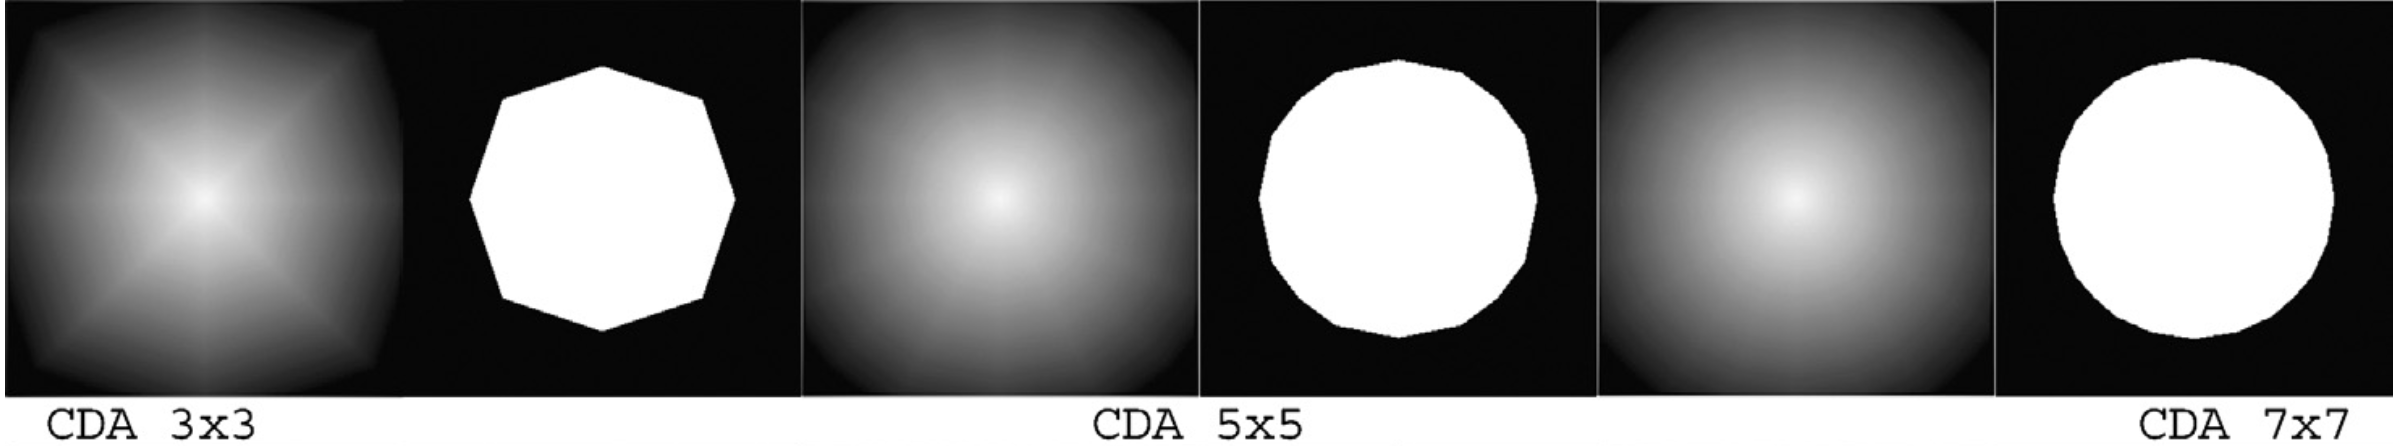
\includegraphics{graphics/df/multi-distance-transform}
	\caption{Results of various distance transform algorithms applied to an input test image containing an object consisting of a single point at the center of the image. The result of a perfect distance transform should be circular for this particular input image.}
	\label{f:multi-distance-transform}
\end{figure*}

The "dead reckoning" signed distance transform, by George J. Grevera\cite[40.0mm]{a:dead-reckoning}, which given a modification to the Chamfer distance transform algorithm that allows it to produce more accurate results without increasing the window size. 

\textit{Vector distance transform}, which is also called \textit{Euclidean distance transform}, where each processed voxel stores a vector to its nearest surface point and the vector at an unprocessed voxel is computed from the vectors at its neighbours by means of a \textit{vector template}.

All chamfer distance transform are some degree approximation of vector distance transform. Vector transform can give the exact results, paper \cite{a:Euclidean-Distance-Mapping} and \cite[5mm]{a:Vector-City-VDT} gives more details. Distance transform has been used in image processing widely.


\section{Representation of Distance Fields}
A 3-dimension distance fields could be stored in a volume texture in GPU, but that's can be can be memory consuming. In the game scene, the world can be infinity, and there are also large empty space in the sky or the house. Hence, there is a great incentive to develop more parsimonious representations which adapter better.

In this section, we mainly introduce two group of techniques: \textit{adaptive distance fields} and \textit{complete distance fields}, due to its widely adopted and its characteristic. There are some variations, but we only discuss the basic idea behind them.

\section{Adaptive Distance field}
Since regularly sampled distance field has the aforementioned drawbacks, many approaches use a hierarchical grid, in which the most empty space can be ignored. Moreover, fine detail requires dense sampling. and immense volumes are needed to accurately represent.

\textit{adaptive distance fields, ADFs}\cite{a:adf} use adaptive, detail-directed sampling, with high sampling rates in regions where the distance field contains fine detail and low sampling rates where the field varies smoothly. Adaptive sampling permits arbitrary accuracy in the reconstructed field together with efficient memory usage. 

In order to process the adaptively sampled data more efficiently, ADFs use a Octree data structure. Here demonstrate the concept in 2D (with quadtrees), in a quadtree-based ADF, each quadtree cell contains the sampled distance values of the cell's 4 corners and pointers to parent and child cells.
 
\begin{figure*}
	\begin{subfigure}[b]{0.5\textwidth}
		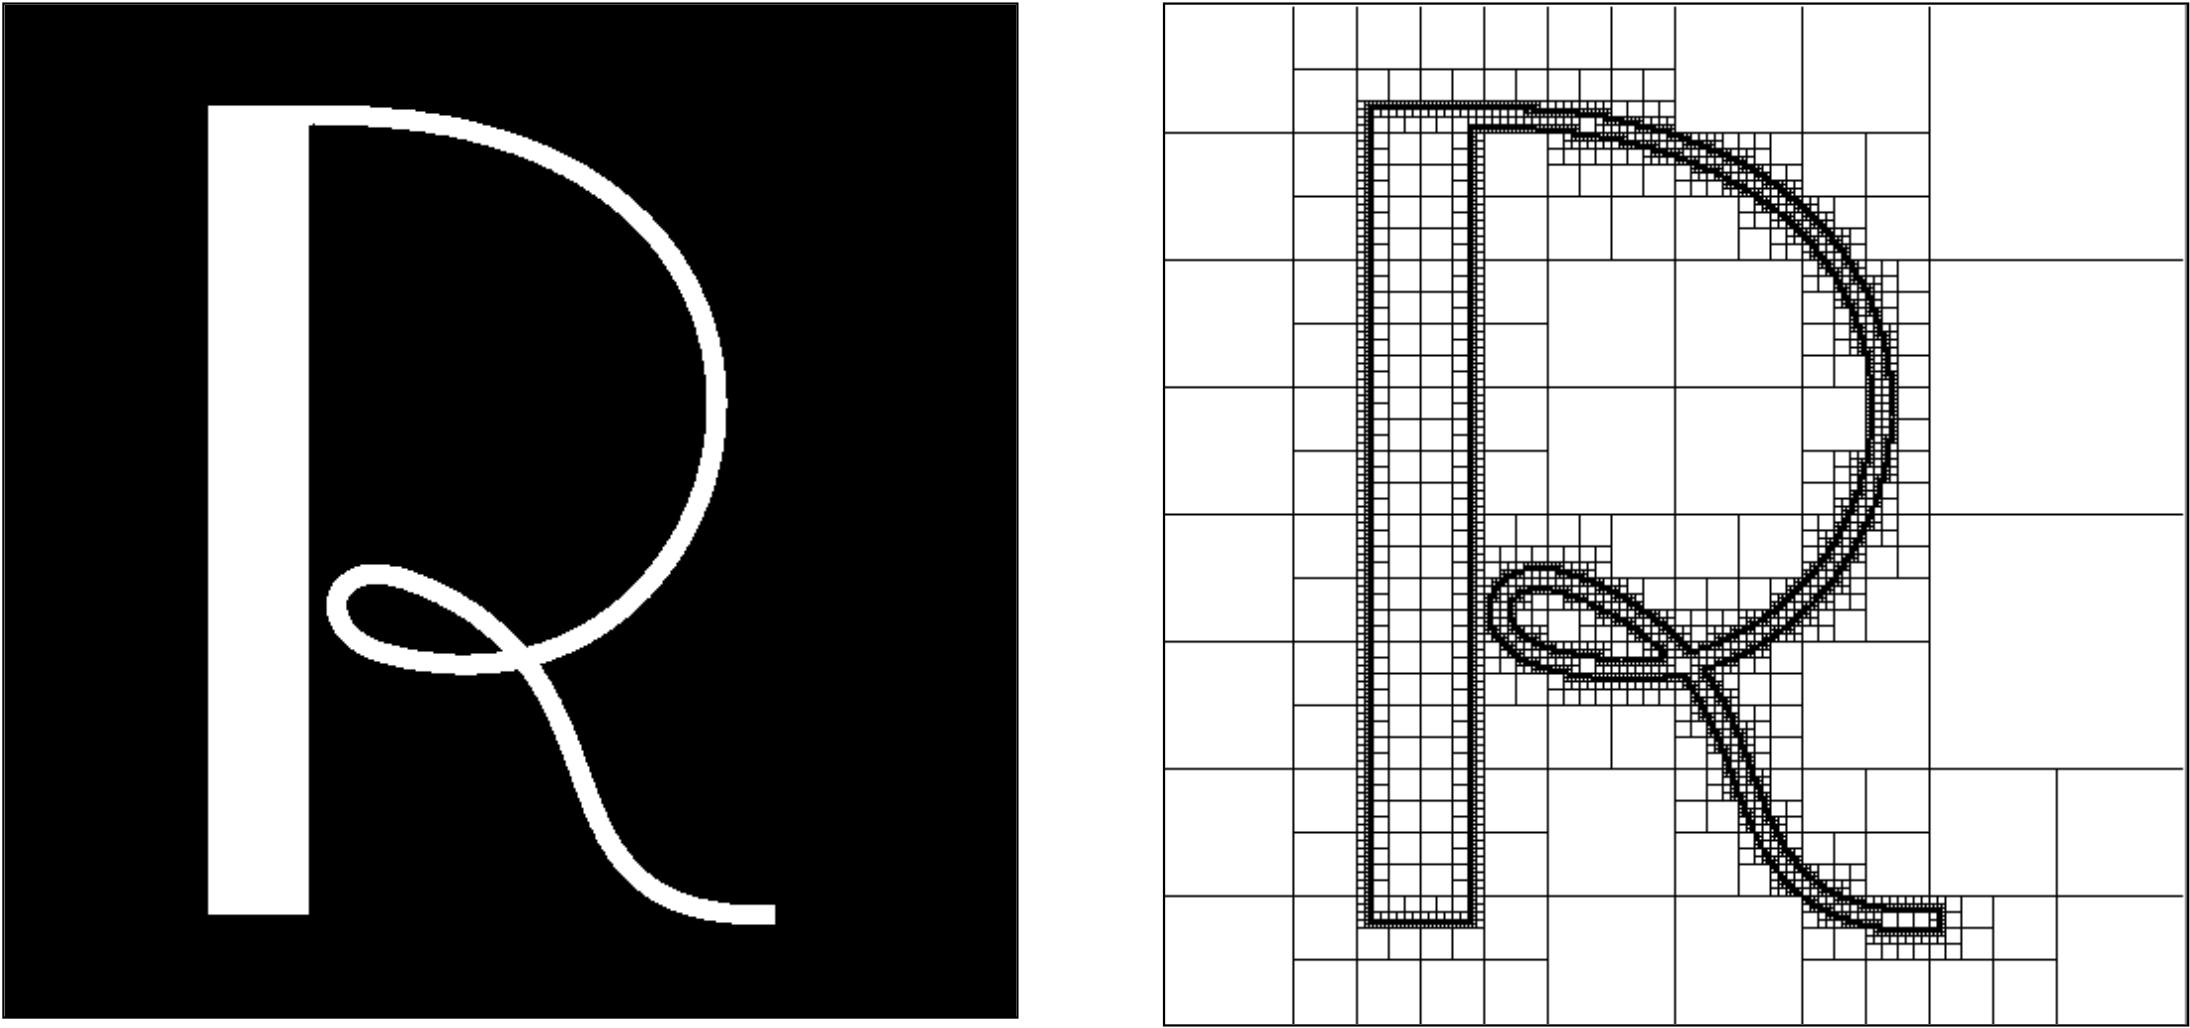
\includegraphics{graphics/df/adf-1}
		\caption{"R" and 3-color quadtree containing 23,573 cells.}
	\end{subfigure}
	\begin{subfigure}[b]{0.5\textwidth}
		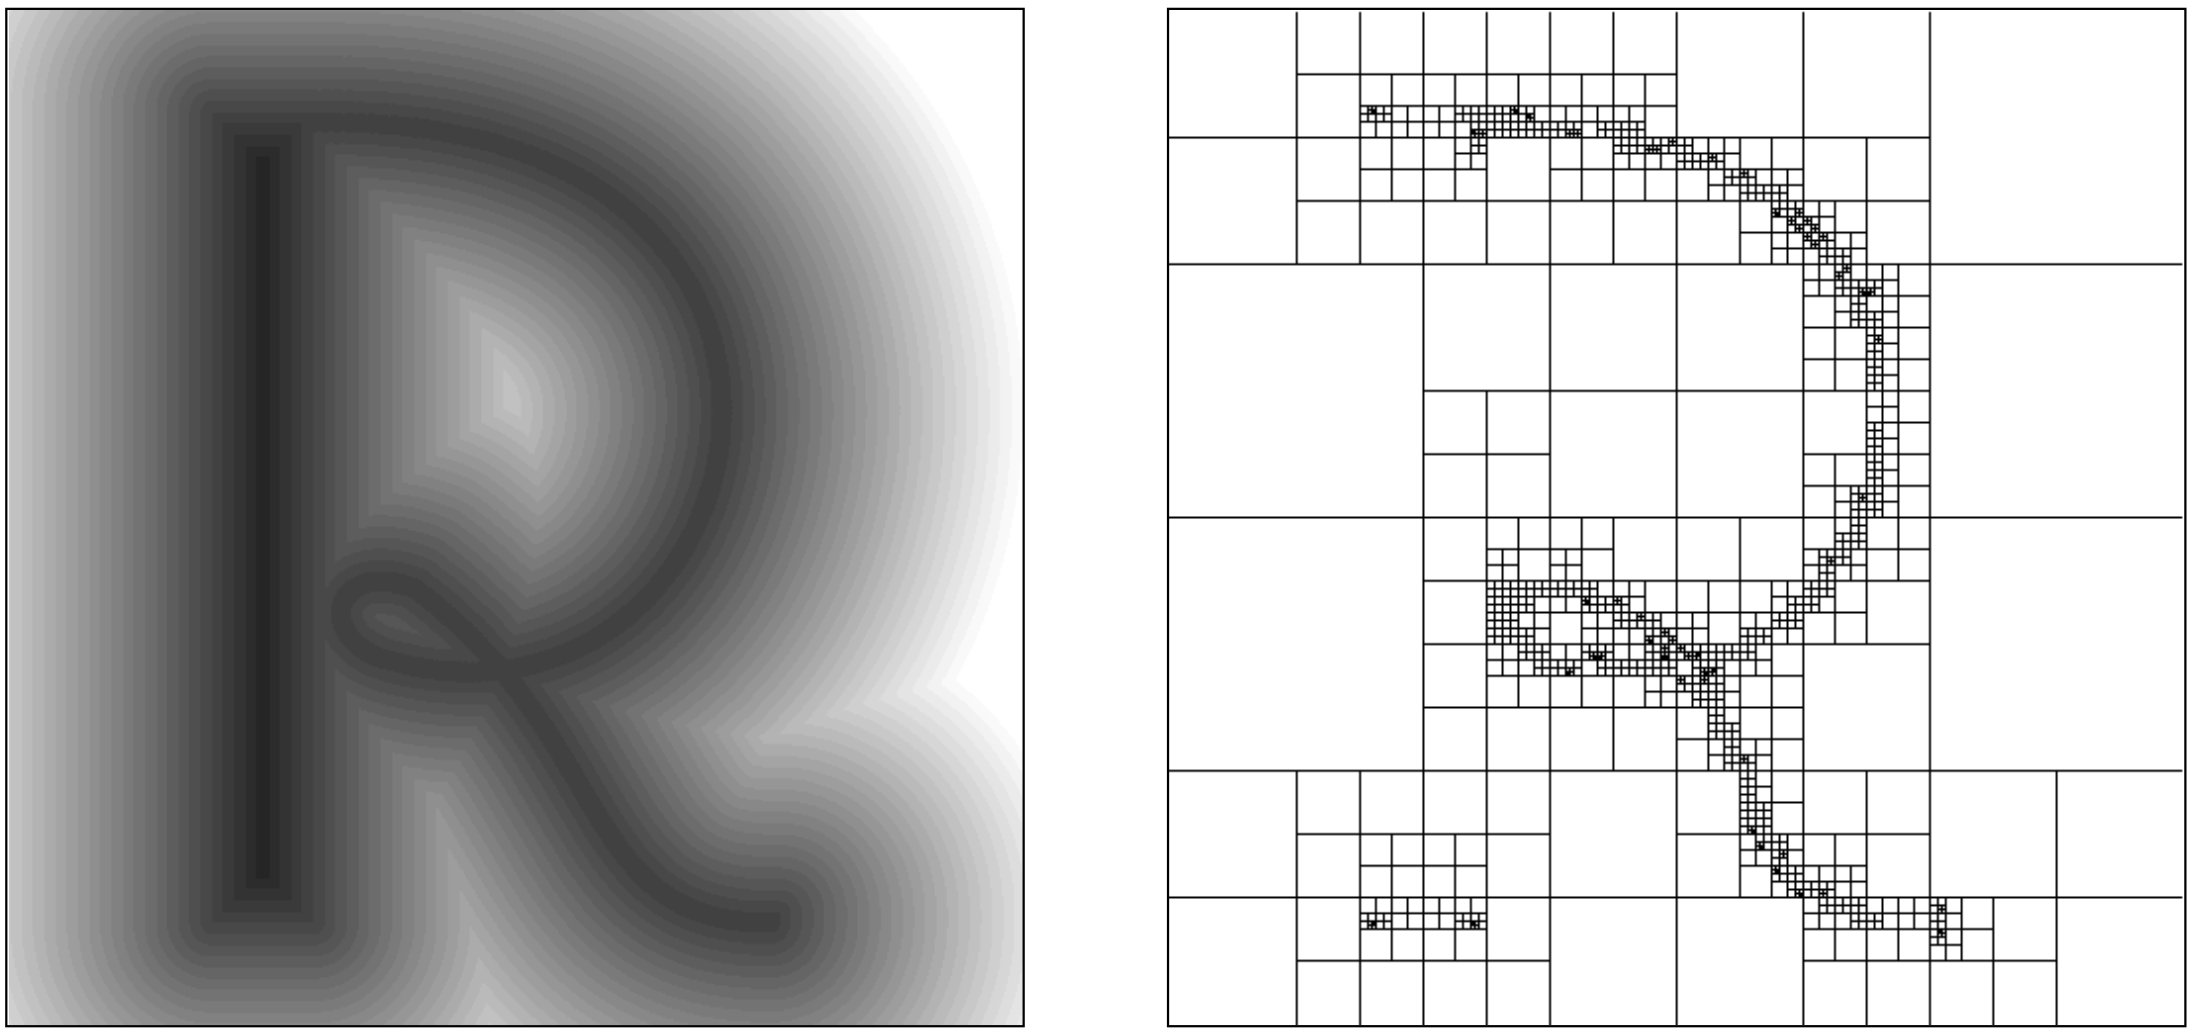
\includegraphics{graphics/df/adf-2}
		\caption{Distance field of "R" and ADF containing 1713 cells.}
	\end{subfigure}
	\caption{Comparison of triangle count for "R" to ADF size.}
	\label{f:adf}
\end{figure*}

Given a shape in figure \ref{f:adf}, subdivision of a cell in the quadtree depends on the variation of the distance field over the parent cell. This differs from 3-color quadtrees which represent object boundaries by assigning one of the three types to each cell in the quadtree: interior, exterior and boundary. 

In 3-color quadtrees, all boundary cells are subdivided to a predetermined highest resolution level. In contrast, boundary cells of ADFs are only subdivided when the distance field within a cell is not well approximated by bilinear interpolation of its corner values. Hence, large cells can be used to represent edges in regions where the shape is relatively smooth, resulting in significantly more compression than 3-color quadtrees.

The Generation of an ADFs requires a procedure or function to produce the distance function, which we can use the previous section's method to generate the distance fields.    

\begin{figure*}
	\begin{subfigure}[b]{0.5\textwidth}
		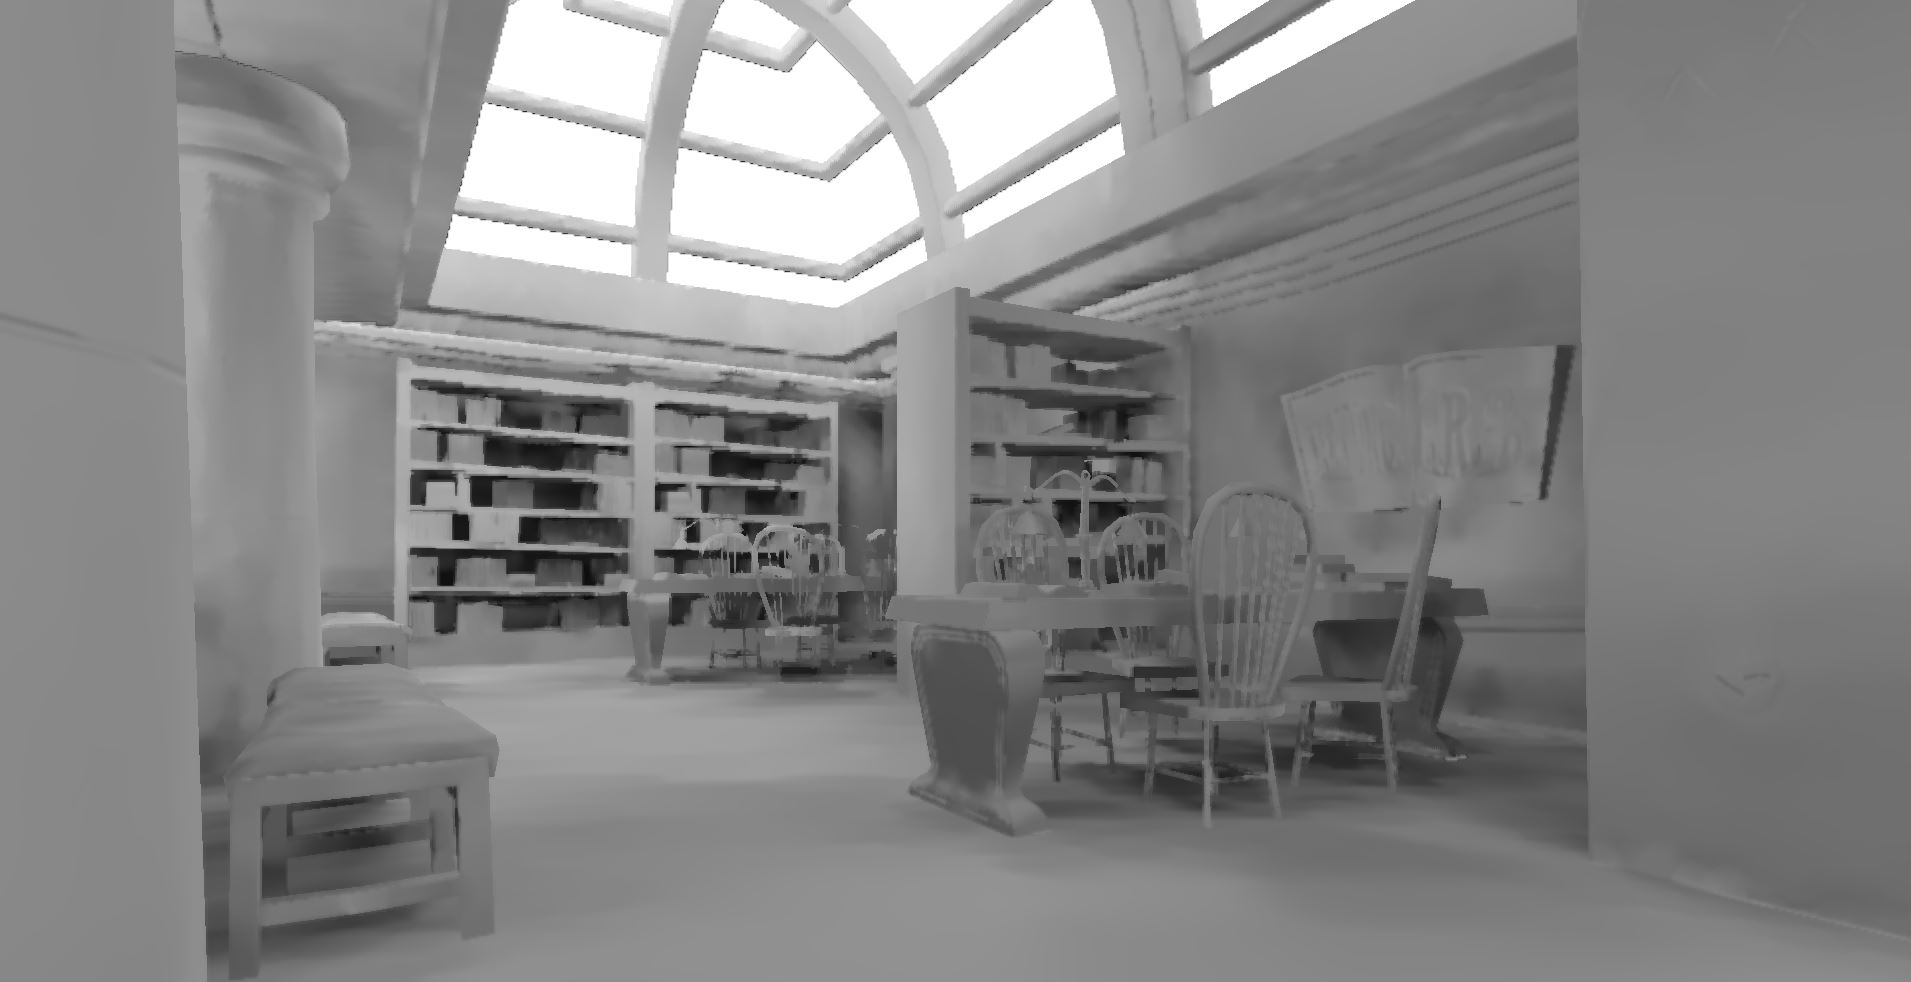
\includegraphics{graphics/df/DFAO_View_OldMethod}
		\caption{Ambient occlusion with ADFs.}
	\end{subfigure}
	\begin{subfigure}[b]{0.5\textwidth}
		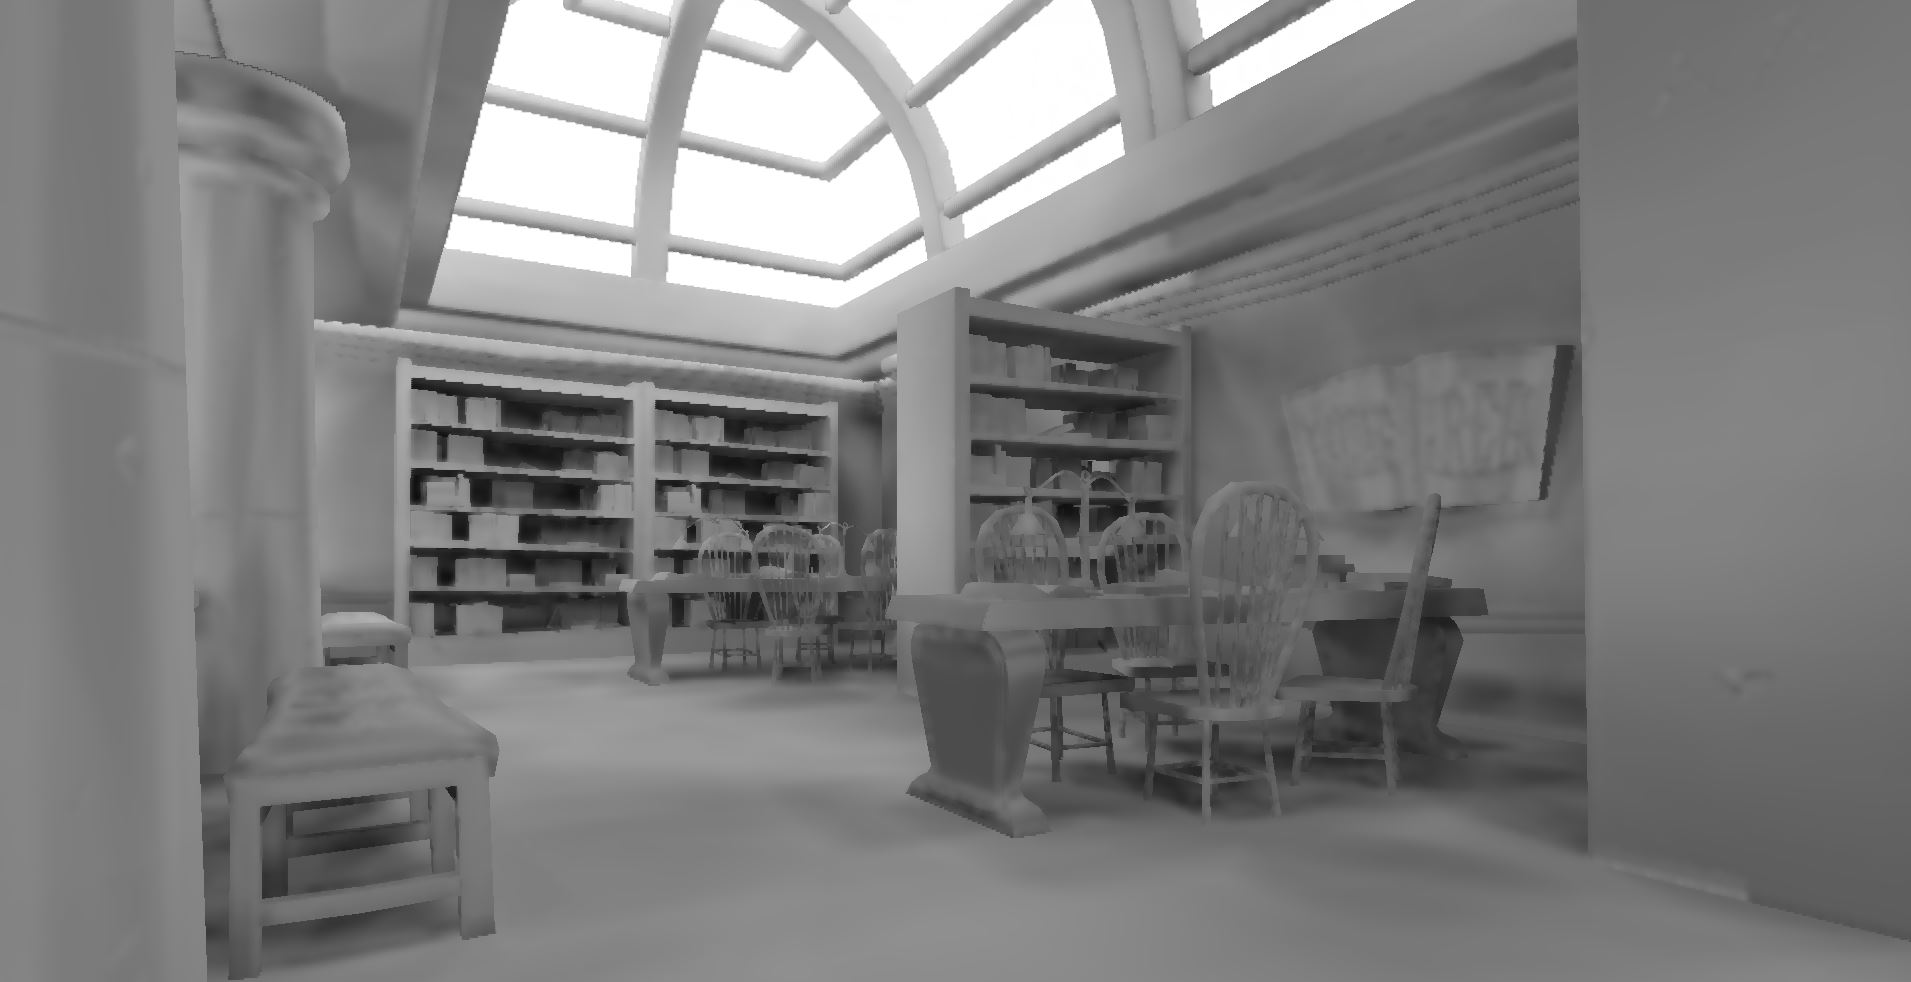
\includegraphics{graphics/df/DFAO_View_NewMethod}
		\caption{Ambient occlusion with a smoother method.}
	\end{subfigure}
	\begin{subfigure}[b]{0.5\textwidth}
		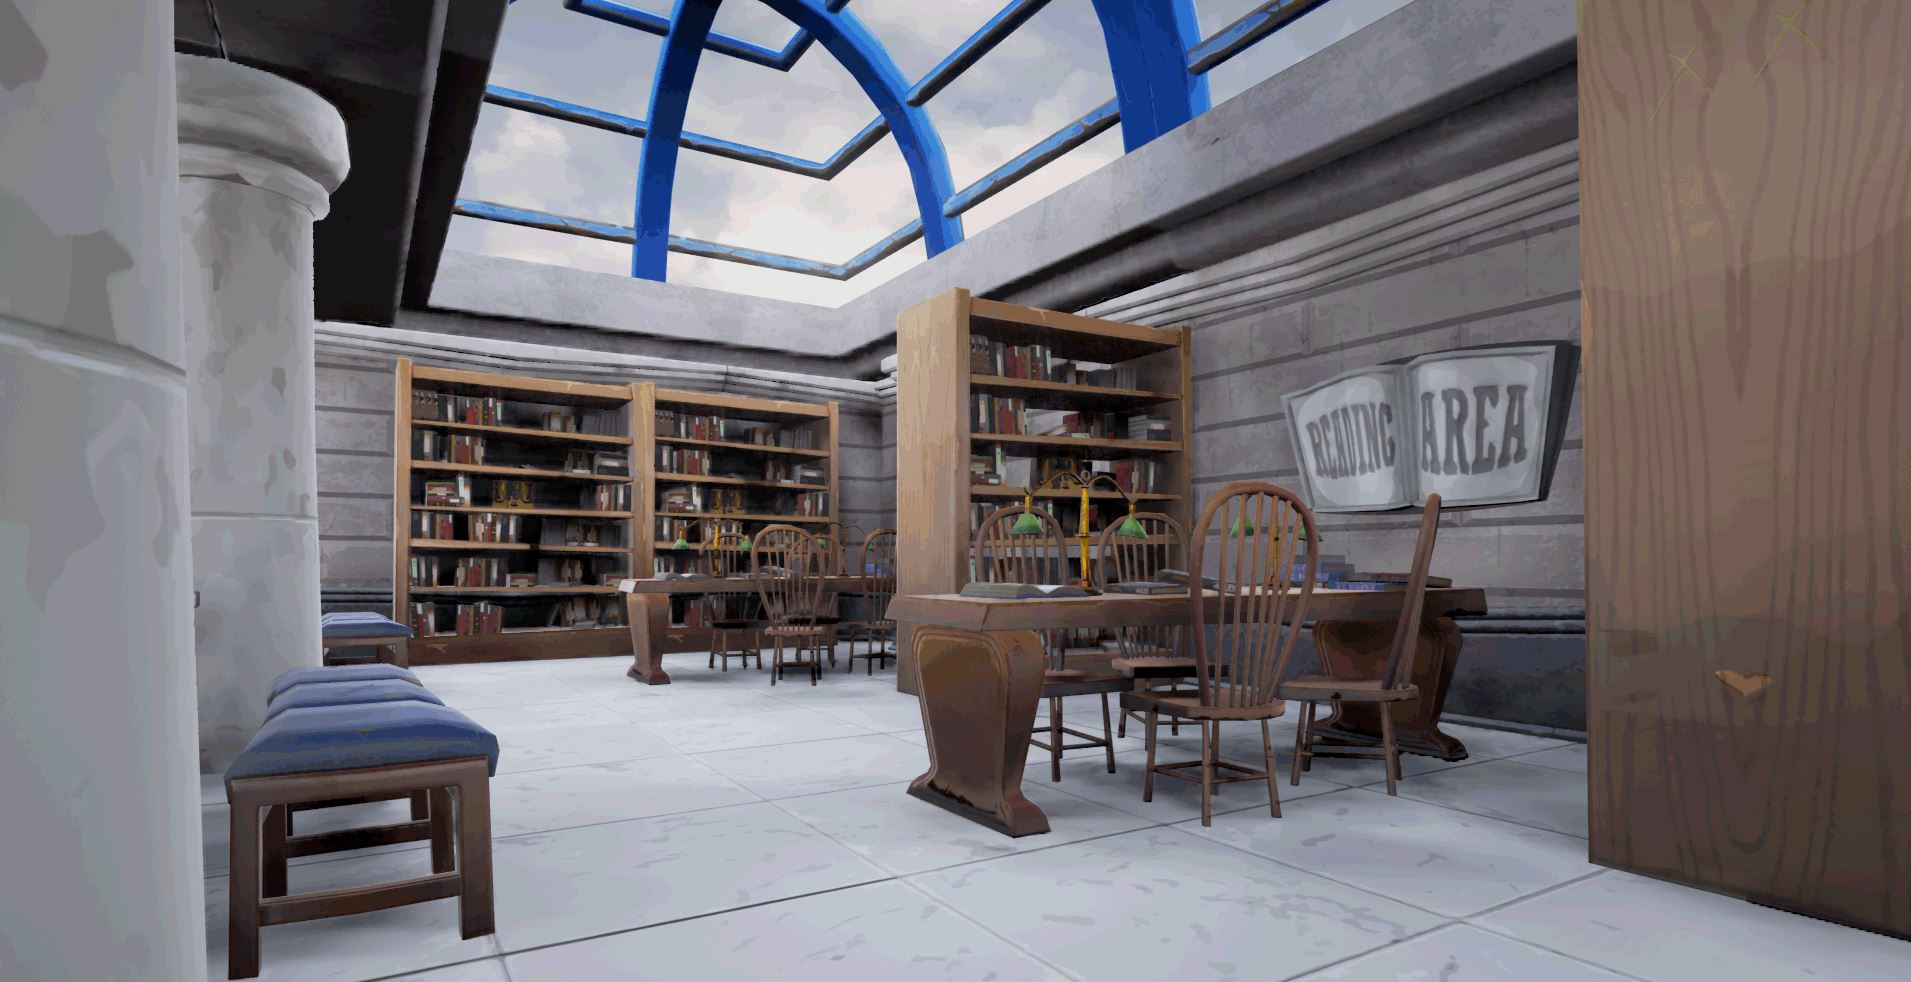
\includegraphics{graphics/df/DFAO_Scene_OldMethod}
		\caption{Render result use (a).}
	\end{subfigure}
	\begin{subfigure}[b]{0.5\textwidth}
		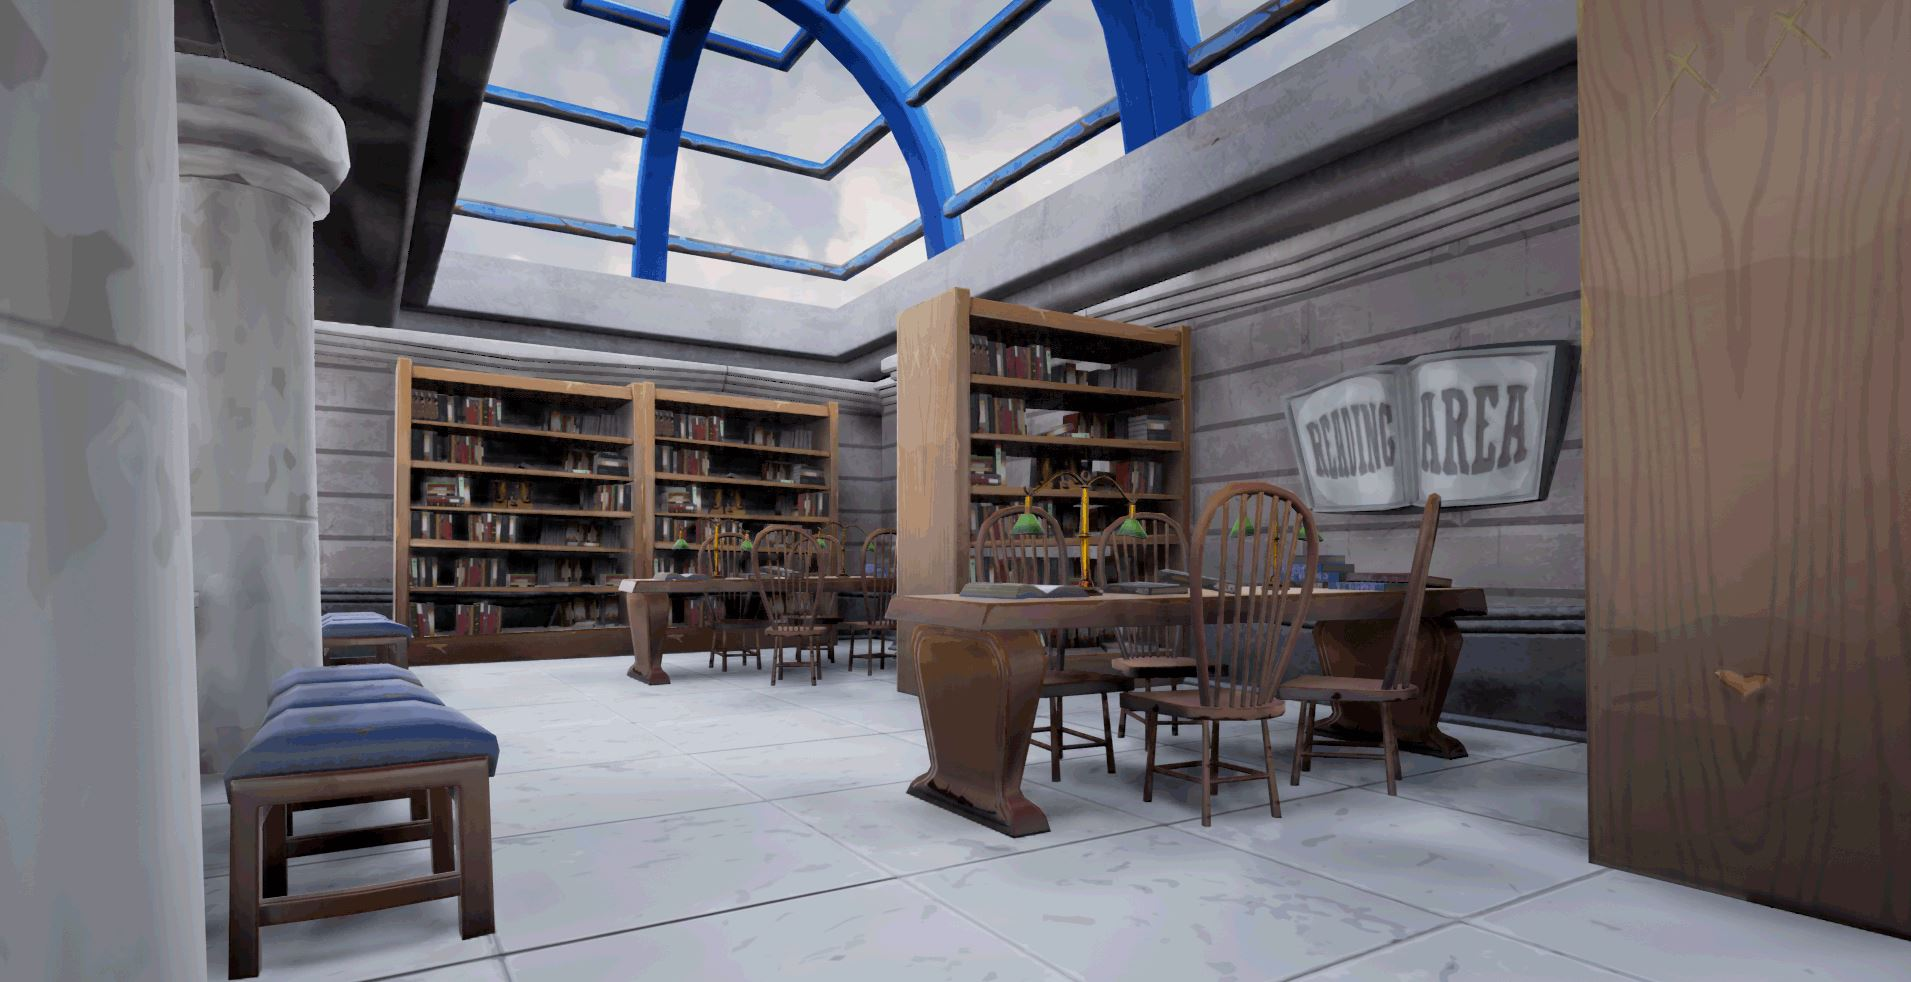
\includegraphics{graphics/df/DFAO_Scene_NewMethod}
		\caption{Render result use (b).}
	\end{subfigure}
	\caption{Comparison of ADFs and some smoother methods. In Unreal Engine 4 due to its caused a lot if splotchiness in clean environment, they have abandoned ADFs (but I don't know what their new method is)(Images courtesy of Epic Games).}
	\label{f:ue4-adf-problem}
\end{figure*}

Although it's efficiently memory usage, ADFs have some drawbacks. Due to its adaptive sampling, so flat surfaces did less work, this also caused a lot of splotchiness in clean environments. Figure \ref{f:ue4-adf-problem} shows the difference between use ADF and other smooth approaches in ambient occlusion (which we will discuss in this article). This leads us to discover some more smooth methods.



\section{Complete Distance Field}
Due to Nyquist's Law\footnote{The sampling rate must be at least two times the highest frequency component in the signal.}, no existing volumetric methods based on the linear sampling theory can fully capture surface details, such as corners and edges, in 3D space. \textit{Complete distance field representation} does not rely on Nyquist's sampling theory, by constructing a volume where each voxel has a complete description of all portions of surface that affect the local distance field.

\textit{Complete distance field representation (CDFR)}\cite{a:A-Complete-Distance-Field-Representation} has a complete distance definition, which is really disparate from the theory of linear sampling\footnote{Which is also called point-based approach, which use a single discrete voxel represent a distance, by the paper CDFR. Like the textures in GPU which every single texel represent a color and the shader calculate a pixel by filtering the texels, the point-based approach calculate the distance by filtering the neighbour's values. CDFR does not rely on filtering. So ADF is a point-based approach. but CDFR algorithm can be embedded into the ADF structure for an exact distance field representation that is efficient both in terms of storage and processing time.}. Once the distance volume is constructed, we can extract any distance contour to any requirement of accuracy. 

CDFR based on some observations. For instance, suppose in a 1-dimensional space, we have an impulse. It’s frequency components extend to infinity. There is no way to use a finite sampling frequency to sample the impulse without aliasing. But on the other hand, as illustrated in Fig \ref{f:1-dimension-space}, the signed distance field of the impulse is a linear function which extends from negative infinity to positive infinity. Sampling this linear function can be accurate with a relatively low sampling rate.

To capture the exact location of the impulse in figure \ref{f:1-dimension-space}, we do not have to use sampling. Alternatively, all one needs is to place an anchor point at some location, and record the signed distance from the anchor to the impulse. In this method, preserving the exact position of the impulse is made straight-forward. This observation motivated our research towards a new distance representation for distance fields.

\begin{figure}
	\begin{center}
		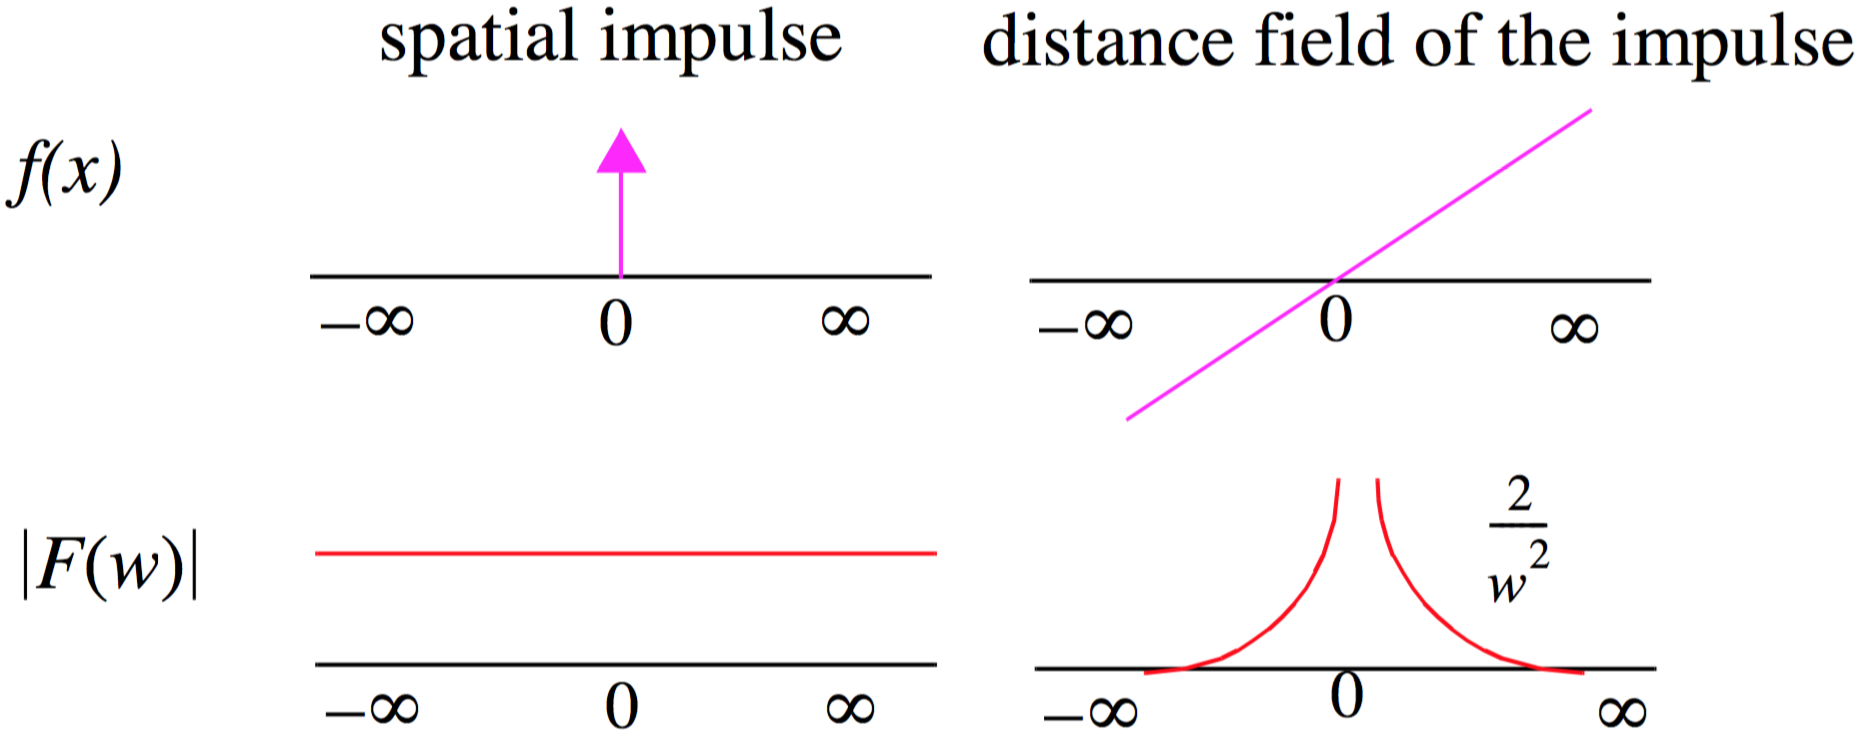
\includegraphics[width=0.75\textwidth]{graphics/df/1-dimension-space}
	\end{center}
	\caption{Without low-pass filtering, it's impossible to sample the impulse(lest), but we can sample its distance field(right).}
	\label{f:1-dimension-space}
\end{figure}

A \textit{complete distance definition (CDD)} is a set of parameters describing both the distance from a 3D point to a surface geometry primitive and the geometry primitive itself. Specifically, when the shape is represented as a mesh of triangles, CDD reduces to a tuple that consists of a scalar canonical distance value, and a description of the triangle with a vertex list and an edge list:

\begin{equation}
	<distance, <v_{1},v_{2},v_{3}>, <e_{1},e_{2},e_{3}>>
\end{equation}

\begin{figure}
\sidecaption
	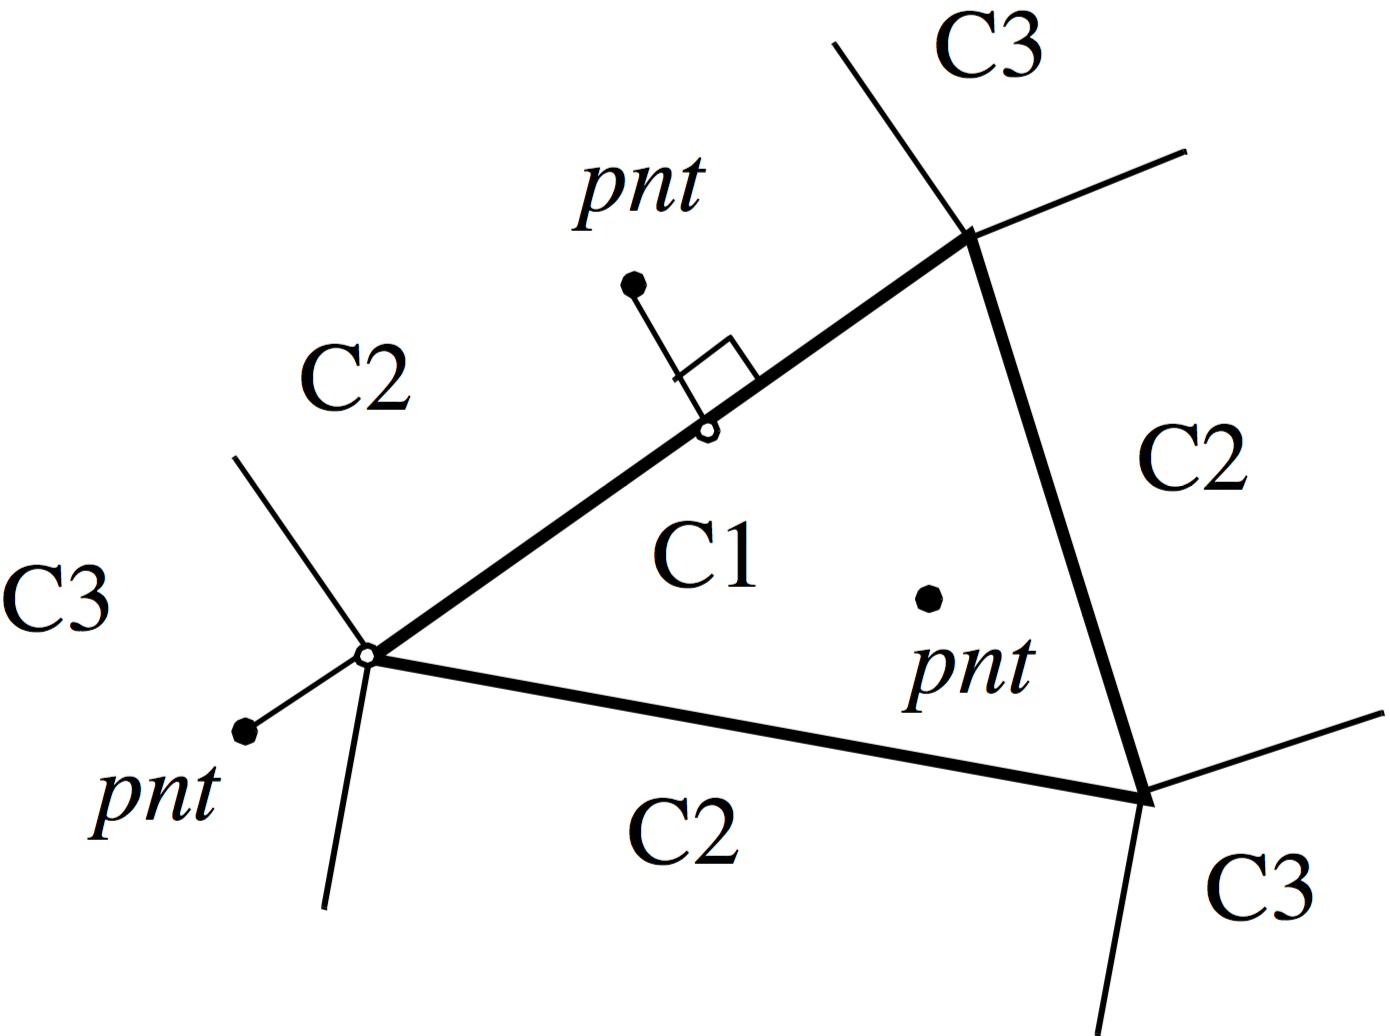
\includegraphics[width=0.65\textwidth]{graphics/df/complete-distance-definition}
	\caption{If $pnt$ projects into $tri$, it's case $C_{1}$. Otherwise, $pnt$ is either $C_{2}$ or $C_{3}$, depending on whether it's closer to an edge or a vertex. This diagram is drawn in 2D for ease of illustration.}
	\label{f:complete-distance-definition}
\end{figure}

The value \textit{distance} is the true Euclidean distance from the voxel center to a finite triangle. The values of $<v_{1},v_{2},v_{3}>$ and $<e_{1},e_{2},e_{3}>$ formed a \textit{base triangle}, which is used to determine the sign, by using the outward normal direction of the base triangle and the relative position of $pnt$, we can determine the sign of the distance at $pnt$ without ambiguity.

For a triangle and a 3D point $pnt$, if $pnt$ orthogonally projects into $C_{1}$, see figure \ref{f:complete-distance-definition}, the distance is the length from $pnt$ to the plane $tri$ and $C_{1}$ become the \textit{based triangle} of $pnt$; Otherwise, if $pnt$ orthogonally projects into any of the three edges, then the distance is the shortest distance from $pnt$ to an edge that $pnt$ projects orthogonally onto, and between the two triangles sharing that edge, the triangle with a normal direction closer to $V$'s direction is $pnt$'s \textit{base triangle}; Similarly, in $C_{3}$ case we can find the shortest vertexes as distance, and one of $C_{1}$ and $C_{3}$ as the \textit{base triangle}.

Then we can use CDD to build a complete distance field representation. which allowing exact capture of all geometric details to any level of accuracy.

Give a surface mesh, in the voxelization step, we store CDD tuple with each surface voxel, rather than single value distances.

\begin{figure}
	\begin{center}
		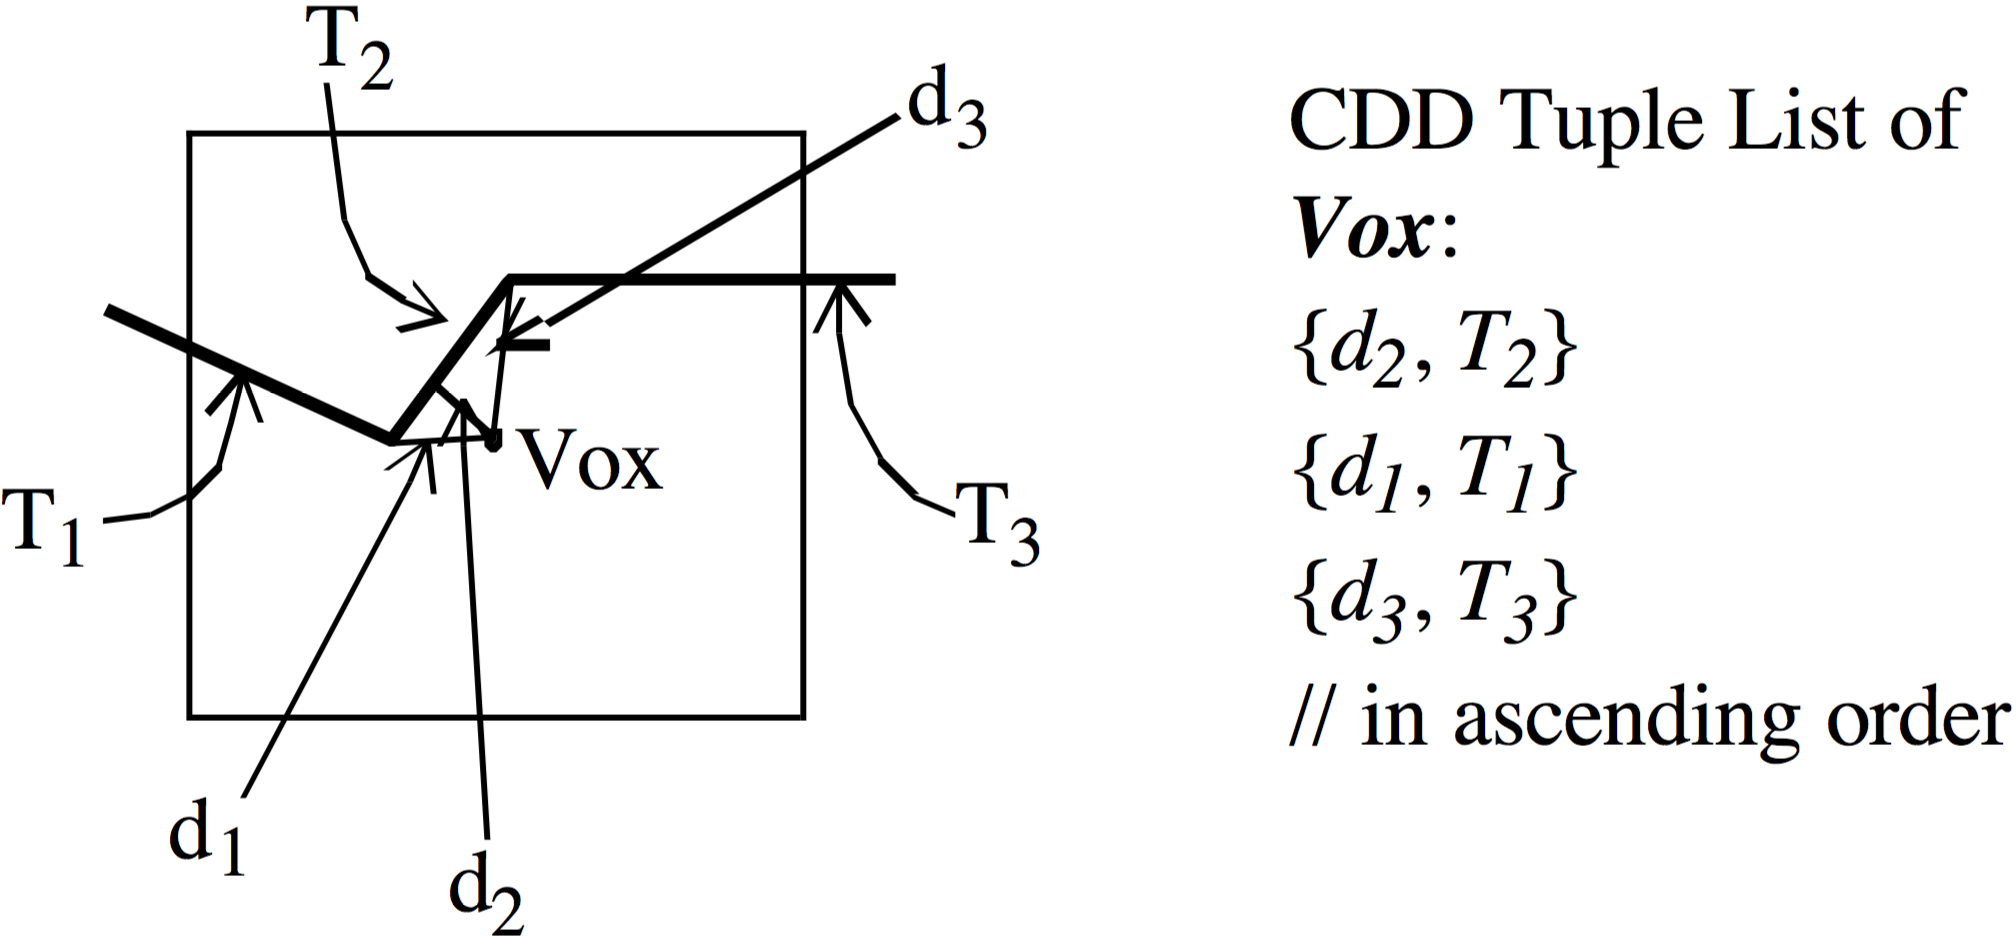
\includegraphics[width=0.65\textwidth]{graphics/df/cdd-tuple-list}
	\end{center}
	\caption{A 2D illumination of building a CDD tuple list for a surface voxel, $Vol$. There are 3 triangles intersecting $Vox$. The CDD tuple list is organized in ascending distance order, with the minimal distance of $Vox$ being $d_{2}$.}
	\label{f:cdd-tuple-list}
\end{figure}

For each triangle touching a surface voxel, a CDD tuple is stored with that voxel. The end result of the voxelization step leaves all surface voxels with a list of CDD tuples, sorted in ascending order by distance values. Figure \ref{f:cdd-tuple-list} provides an example of voxelizing a single surface voxel, $Vox$. There are three triangles touching Vox. T2 is case $C_1$, with $T_1$ and $T_3$ being case $C_{2}$ or $C_{3}$. The minimal distance of Vox, measured from the center of Vox is $d_2$. As a result, Vox has a sorted list of 3 CDD tuples.
At the end of voxelization, we have a volume where each voxel which the surface intersects contains a list of polygons cutting through it.









